% Options for packages loaded elsewhere
\PassOptionsToPackage{unicode}{hyperref}
\PassOptionsToPackage{hyphens}{url}
\PassOptionsToPackage{dvipsnames,svgnames,x11names}{xcolor}
%
\documentclass[
  12pt,
]{article}

\usepackage{amsmath,amssymb}
\usepackage{setspace}
\usepackage{iftex}
\ifPDFTeX
  \usepackage[T1]{fontenc}
  \usepackage[utf8]{inputenc}
  \usepackage{textcomp} % provide euro and other symbols
\else % if luatex or xetex
  \usepackage{unicode-math}
  \defaultfontfeatures{Scale=MatchLowercase}
  \defaultfontfeatures[\rmfamily]{Ligatures=TeX,Scale=1}
\fi
\usepackage{lmodern}
\ifPDFTeX\else  
    % xetex/luatex font selection
  \setmainfont[]{Times New Roman}
\fi
% Use upquote if available, for straight quotes in verbatim environments
\IfFileExists{upquote.sty}{\usepackage{upquote}}{}
\IfFileExists{microtype.sty}{% use microtype if available
  \usepackage[]{microtype}
  \UseMicrotypeSet[protrusion]{basicmath} % disable protrusion for tt fonts
}{}
\makeatletter
\@ifundefined{KOMAClassName}{% if non-KOMA class
  \IfFileExists{parskip.sty}{%
    \usepackage{parskip}
  }{% else
    \setlength{\parindent}{0pt}
    \setlength{\parskip}{6pt plus 2pt minus 1pt}}
}{% if KOMA class
  \KOMAoptions{parskip=half}}
\makeatother
\usepackage{xcolor}
\usepackage[margin=1in]{geometry}
\setlength{\emergencystretch}{3em} % prevent overfull lines
\setcounter{secnumdepth}{-\maxdimen} % remove section numbering
% Make \paragraph and \subparagraph free-standing
\ifx\paragraph\undefined\else
  \let\oldparagraph\paragraph
  \renewcommand{\paragraph}[1]{\oldparagraph{#1}\mbox{}}
\fi
\ifx\subparagraph\undefined\else
  \let\oldsubparagraph\subparagraph
  \renewcommand{\subparagraph}[1]{\oldsubparagraph{#1}\mbox{}}
\fi


\providecommand{\tightlist}{%
  \setlength{\itemsep}{0pt}\setlength{\parskip}{0pt}}\usepackage{longtable,booktabs,array}
\usepackage{calc} % for calculating minipage widths
% Correct order of tables after \paragraph or \subparagraph
\usepackage{etoolbox}
\makeatletter
\patchcmd\longtable{\par}{\if@noskipsec\mbox{}\fi\par}{}{}
\makeatother
% Allow footnotes in longtable head/foot
\IfFileExists{footnotehyper.sty}{\usepackage{footnotehyper}}{\usepackage{footnote}}
\makesavenoteenv{longtable}
\usepackage{graphicx}
\makeatletter
\def\maxwidth{\ifdim\Gin@nat@width>\linewidth\linewidth\else\Gin@nat@width\fi}
\def\maxheight{\ifdim\Gin@nat@height>\textheight\textheight\else\Gin@nat@height\fi}
\makeatother
% Scale images if necessary, so that they will not overflow the page
% margins by default, and it is still possible to overwrite the defaults
% using explicit options in \includegraphics[width, height, ...]{}
\setkeys{Gin}{width=\maxwidth,height=\maxheight,keepaspectratio}
% Set default figure placement to htbp
\makeatletter
\def\fps@figure{htbp}
\makeatother
% definitions for citeproc citations
\NewDocumentCommand\citeproctext{}{}
\NewDocumentCommand\citeproc{mm}{%
  \begingroup\def\citeproctext{#2}\cite{#1}\endgroup}
\makeatletter
 % allow citations to break across lines
 \let\@cite@ofmt\@firstofone
 % avoid brackets around text for \cite:
 \def\@biblabel#1{}
 \def\@cite#1#2{{#1\if@tempswa , #2\fi}}
\makeatother
\newlength{\cslhangindent}
\setlength{\cslhangindent}{1.5em}
\newlength{\csllabelwidth}
\setlength{\csllabelwidth}{3em}
\newenvironment{CSLReferences}[2] % #1 hanging-indent, #2 entry-spacing
 {\begin{list}{}{%
  \setlength{\itemindent}{0pt}
  \setlength{\leftmargin}{0pt}
  \setlength{\parsep}{0pt}
  % turn on hanging indent if param 1 is 1
  \ifodd #1
   \setlength{\leftmargin}{\cslhangindent}
   \setlength{\itemindent}{-1\cslhangindent}
  \fi
  % set entry spacing
  \setlength{\itemsep}{#2\baselineskip}}}
 {\end{list}}
\usepackage{calc}
\newcommand{\CSLBlock}[1]{\hfill\break\parbox[t]{\linewidth}{\strut\ignorespaces#1\strut}}
\newcommand{\CSLLeftMargin}[1]{\parbox[t]{\csllabelwidth}{\strut#1\strut}}
\newcommand{\CSLRightInline}[1]{\parbox[t]{\linewidth - \csllabelwidth}{\strut#1\strut}}
\newcommand{\CSLIndent}[1]{\hspace{\cslhangindent}#1}

\usepackage{fontspec}
\usepackage{multirow}
\usepackage{multicol}
\usepackage{colortbl}
\usepackage{hhline}
\newlength\Oldarrayrulewidth
\newlength\Oldtabcolsep
\usepackage{longtable}
\usepackage{array}
\usepackage{hyperref}
\usepackage{float}
\usepackage{wrapfig}
% Load titlesec package to customize heading styles
\usepackage{titlesec}

% SAA Heading Style: Level 1 (Centered, Bold, No Number)
\titleformat{\section}{\normalfont\bfseries\filcenter}{}{0em}{}[\vspace{1em}]

% SAA Heading Style: Level 2 (Flush-left, Bold, No Number)
\titleformat{\subsection}{\normalfont\bfseries}{}{0em}{}

% SAA Heading Style: Level 3 (Flush-left, Italic, No Number)
\titleformat{\subsubsection}{\normalfont\itshape}{}{0em}{}

% Remove all section numbering
\setcounter{secnumdepth}{0}

% Customize caption format to "Figure 1." and "Table 1."
\usepackage[labelfont=bf,labelsep=period]{caption}
\makeatletter
\@ifpackageloaded{caption}{}{\usepackage{caption}}
\AtBeginDocument{%
\ifdefined\contentsname
  \renewcommand*\contentsname{Table of contents}
\else
  \newcommand\contentsname{Table of contents}
\fi
\ifdefined\listfigurename
  \renewcommand*\listfigurename{List of Figures}
\else
  \newcommand\listfigurename{List of Figures}
\fi
\ifdefined\listtablename
  \renewcommand*\listtablename{List of Tables}
\else
  \newcommand\listtablename{List of Tables}
\fi
\ifdefined\figurename
  \renewcommand*\figurename{Figure}
\else
  \newcommand\figurename{Figure}
\fi
\ifdefined\tablename
  \renewcommand*\tablename{Table}
\else
  \newcommand\tablename{Table}
\fi
}
\@ifpackageloaded{float}{}{\usepackage{float}}
\floatstyle{ruled}
\@ifundefined{c@chapter}{\newfloat{codelisting}{h}{lop}}{\newfloat{codelisting}{h}{lop}[chapter]}
\floatname{codelisting}{Listing}
\newcommand*\listoflistings{\listof{codelisting}{List of Listings}}
\makeatother
\makeatletter
\makeatother
\makeatletter
\@ifpackageloaded{caption}{}{\usepackage{caption}}
\@ifpackageloaded{subcaption}{}{\usepackage{subcaption}}
\makeatother
\ifLuaTeX
  \usepackage{selnolig}  % disable illegal ligatures
\fi
\usepackage{bookmark}

\IfFileExists{xurl.sty}{\usepackage{xurl}}{} % add URL line breaks if available
\urlstyle{same} % disable monospaced font for URLs
\hypersetup{
  pdftitle={Hire Ed: Job Market Dynamics for Tenure-Track Faculty Positions in Archaeology},
  pdfauthor={Ben Marwick1,; Anne Marie Poole1; Ailin Zhang1; Setareh Shafizadeh1; Jess Beck2},
  pdfkeywords={archaeology; hiring; academia; job ads},
  colorlinks=true,
  linkcolor={blue},
  filecolor={Maroon},
  citecolor={Blue},
  urlcolor={Blue},
  pdfcreator={LaTeX via pandoc}}

\title{Hire Ed: Job Market Dynamics for Tenure-Track Faculty Positions
in Archaeology}
\author{}
\date{July 8, 2025}

\begin{document}
\maketitle
\begin{abstract}
Many archaeology graduate students pursue advanced degrees in the hope
of undertaking an academic career. Job listing websites often serve as
the first port-of-call for students seeking academic positions. We
examined tenure-track job advertisements over the past decade to gain
insights into the academic job market for archaeologists. Using data
from the community-edited Academic Jobs Wiki for Archaeology, we
examined changes in the academic job market over time. We investigated
the editing dynamics of the Wiki to understand its users and their
biases. We then analyzed the text of 431 job ads posted from 2013--2023.
Our analysis addresses the question of how archaeological topics,
methods, and geographic regions specified in archaeological job ads have
shifted over time. We also explored whether the labor burden for
applicants has changed over time: do institutions request more
information and documents from applicants at the initial stages of
application, compared to a decade ago? Finally, we assessed the
influence of socio-political factors on the changing focus of research
topics in the field. We conclude with implications for archaeology
students, graduates, and advisors seeking to understand the dynamics of
the academic job market and the requirements of employers.
\end{abstract}

\begin{titlepage}
    \centering
    \vspace*{\stretch{1.0}}
    {\huge\bfseries \thetitle\par}
    \vspace{2cm}
    {\Large \theauthor\par}
    \vspace{1cm}
    \theaffiliation
    \vspace*{\stretch{2.0}}
\end{titlepage}
\doublespacing

\setstretch{2}
\textsuperscript{1} Department of Anthropology, University of
Washington, Seattle, USA\\
\textsuperscript{2} School of Archaeology, University College Dublin,
Ireland

\textsuperscript{*} Correspondence:
\href{mailto:bmarwick@uw.edu}{Ben Marwick
\textless{}bmarwick@uw.edu\textgreater{}}

Keywords: archaeology; hiring; academia; job ads

Attend any workshop, conference, or panel that includes early career
researchers and the conversation will be steered inexorably towards the
academic job market: who is hiring, who has attained a tenure-track
position, and who is out of luck this season. Tenure-track positions are
a type of academic job that typically involve a probationary period
(e.g.~five to seven years) culminating in an evaluation of research,
teaching, and service, that if successful, results in permanent
employment, job security and academic freedom. This obsessive focus on
career trajectories is warranted. As of 2019, 53.5\% of colleges and
universities had replaced tenure-eligible lines with contingent
positions (American Association of University Professors 2022a); today,
71\% of faculty in the U.S. are non-tenure-track (Culver and Kezar
2022). The erosion of permanent jobs in American higher education is
linked to a complex intersection of political and economic factors (Beck
2025), including decreasing federal support for higher education,
concomitant increases in student debt (Gusterson 2017), a pronounced
shift in university investment from faculty to administration (Graeber
2018:162--163), and the growing privatization and market orientation of
scientific research (Mirowski 2011).

These cultural and economic shifts are also well encapsulated by
anecdata; any conversation with a junior scholar will reveal the impact
of these larger professional transformations on personal and
professional trajectories. The first author on this paper has applied to
five academic positions over the course of his career, while the last
author has applied to one hundred. A twenty-fold increase in the number
of applications required to obtain a workable long-term academic
position may seem preposterous, but these changing requirements for
applicants are familiar to anyone who has obtained their PhDs since the
Great Recession of 2008. This competitive landscape has deeper roots
than the last economic crisis; writing more than three decades ago,
Rabinow pinpointed ``an awareness\ldots{} that standards have changed
during the last thirty years and the quantitative and qualitative
demands for entry into the system are immeasurably higher now''
(1992:66).

These higher demands include increased overall productivity, higher
national and international mobility, more time spent in precarious
short-term contracts, and the investment of a greater amount of time and
energy in applying for long-term positions. In their survey of early
career researchers in European archaeology, for example, Brami et
al.~found that 52\% of respondents who had obtained their PhD at least
two years before the survey were on fixed-term contracts, while only 9\%
were in permanent positions (2023:Figure 5). In their words, ``the queue
of eager post-docs hoping for a long-term appointment is getting longer,
as is the average time spent in the `queue'\,'' (2023:239). Ribeiro and
Giamakis emphasize that this demographic comprises an academic precariat
that is essential to the functioning of universities, but consists of a
workforce perpetually ``stranded between employment and unemployment''
(Ribeiro and Giamakis 2023:10).

Junior scholars with faculty ambitions are thus stuck in a double-bind,
forced to funnel their energy into seemingly endless applications for
which they receive little to no feedback and which remain invisible on
their CVs. As Dennis et al.~underscore, early career researchers are
``supplicants''---``There is no way for applicants to point out that the
job ads are taking too much time out of the scholarly community's
collective time bank'' (Dennis et al. 2022:1). Acknowledging the new
reality that applying for academic positions is in and of itself a
full-time job, a growing number of anthropology graduate programmes are
offering professionalization courses that cover the ins and outs of
everything from crafting strong cover letters and CVs to performing well
in long-list interviews and preparing teaching demonstrations. These
courses can provide valuable training in the hidden curriculum of the
academy, but the fact that job applications are so complicated that they
require training to navigate suggests more disciplinary attention should
be paid to the ``market'' as a historically contingent set of cultural
practices. As Rabinow maintains, ``if we want ethical considerations to
play a central role in the articulation of truth and power---and I think
we do---then bringing such considerations into view is the necessary
first step towards recognizing who we are today and setting out on the
road to a better place'' (1992:71).

We argue that to understand the dynamics of hiring in academic
archaeology, we must start at the beginning, with the job ad itself.
There is an abundance of recent work on who does and does not get hired
into tenure-track positions in anthropology and archaeology, but less
scholarship on how those hires unfold. Research on hiring dynamics has
amply demonstrated that \emph{where} you get your PhD has an enormous
impact on if and where you get a tenure-track position (Kawa et al.
2019; Mackie and Rockwell 2023), but how about \emph{what} you study?
Are there topical, methodological, or regional specialties that are in
consistent demand, or is there continual flux generated by intellectual
fads, economic incentives, and political attention? Are job applications
more demanding now than they were in the past, or is this a specious
perception generated by the sheer volume of applications necessary to
obtain a long-term academic position?

To answer these questions, this paper explores the demand-side of the
academic job market for archaeologists in the United States. Our study
had two aims: first, to determine if disciplinary trends could be
discerned in the topical, geographic, and methodological foci of the
positions advertised over a ten-year period, and second, to investigate
how requirements for applicants have changed over time.

\section{Background}\label{background}

The academic job market is a source of uncertainty, for both job seekers
and hiring committees. Job seekers must search for ads that are
well-matched to the skill sets and professional experiences that they
have taken years to cultivate. Hiring committees must sift through tens
to hundreds of applicants in the hope of finding a candidate that meets
all of their needs and helps to realize their visions for their program
and for the discipline. Finding the right candidate for the
position---or the right position for the candidate---is akin to finding
a needle in a haystack.

Among many scholars, there is also a perception that the last three
decades have seen the academic job market become increasingly
competitive. Across the social sciences and humanities, there are fewer
jobs available relative to the number of PhD graduates, and higher
numbers of short-term positions relative to permanent positions (Bessner
and Brenes 2021; Brami et al. 2023; Kawa et al. 2019; Kelsky 2015;
Mackie and Rockwell 2023). This market saturation has arisen in tandem
with increasingly complex application requirements. Many job ads now
solicit specific documents in \emph{addition} to the cover letter and
CV, such as teaching, research, and diversity statements. These
additional documents must be tailored for each application, making the
process of applying for jobs a full-time job of its own.

In American anthropology, the number of doctoral anthropology graduates
has increased by about 70\% over the past 30 years, but the number of
new faculty positions has not increased proportionally (Speakman,
Hadden, Colvin, Cramb, Jones, Jones, Kling, et al. 2018). New faculty
positions have dwindled, in part due to the removal of the Age
Discrimination in Employment Act (ADEA) exemption in 1994 which
prohibited mandatory retirement ages in higher education (Earle and
DelPo Kulow 2014). When combined with the institution of tenure, the
ADEA exemption allowed faculty to stay in their posts for as long as
they liked. The median age for faculty in the U.S. now ranks among the
highest for all professions (Kaskie 2016). In tandem with the gradual
de-investment in American higher education since 1980s (Mirowski 2011)
and the aftershocks of the 2008 recession, the ADEA exemption has
cultivated an environment where new lines are few and far between. Among
biological anthropologists, for example, Passalacqua (2018) found ratios
ranging from 1.21 to 0.82 PhDs to job academic advertisements per year,
concluding that academic positions in biological anthropology are barely
at sustainable levels. This echoes findings from other fields. In
biomedical sciences, there is one tenure-track position in the U.S. for
approximately every 6.3 PhD graduates (Ghaffarzadegan et al. 2015). In
engineering, Larson et al., have calculated that providing jobs for even
50\% of PhD graduates would require the field to expand at an
``improbable'' rate of 14\% per year (2014:747). As they emphasize,
``\ldots{} the system in many places is saturated, far beyond capacity
to absorb new PhDs in academia at the rates they are being produced''
(Larson et al. 2014:749).

PhD graduates who do not go directly into a tenure-track faculty
position after graduation often go into a series of short-term
appointments as part-time or limited contract instructors, also known as
adjunct or contingent faculty. The rising number of contingent faculty
has long been a concern in U.S. higher education (Trevithick 2010). Data
from the American Association of University Professors' 2021--22 faculty
survey indicate that more than 60\% of faculty positions in U.S.
universities were held by non-tenure-track full time or part time
contingent faculty members (American Association of University
Professors 2022b). Contingent faculty positions are precarious because
they provide low or no health and retirement benefits, limited
opportunities for professional development, and lower salaries relative
to tenure-track positions. PhD graduates who have a sequence of
short-term academic positions are often disadvantaged financially due to
low compensation combined with expensive and frequent relocation,
restrictive socially due to isolation from family and community, and
limited professionally due to being ineligible for many decision-making
roles at the universities at which they work (Platzer and Allison 2018).

Success in tenure-track job applications in archaeology is strongly
determined by where applicants get their PhDs. Data from the 2014--2015
AnthroGuide publication of the American Anthropological Association
shows that just ten out of over 100 U.S. graduate programs produced over
30\% of the graduates hired into tenure-track faculty positions
(Speakman, Hadden, Colvin, Cramb, Jones, Jones, Kling, et al. 2018).
Top-ranking programs are placing fewer than one in three graduates in
tenure-track jobs (Mackie and Rockwell 2023). Similarly, a network
analysis of 1,918 faculty holding tenured or tenure-track positions at
PhD-granting anthropology programs in the U.S. in 2015 (including 506
archaeologists) found that the just fifteen graduate programs produced
53 percent of tenured and tenure-track positions (Kawa et al. 2019).
This network analysis showed that programs with large endowments and
widely cited faculty who hold prestigious awards produce the majority of
tenured and tenure-track faculty.

Hiring bias predicated on the prestige of specific institutions and
programs is not unique to anthropology. Targeted studies of sociology,
communication, operations research, and industrial systems engineering
show similar dynamics (Barnett et al. 2010; Castillo et al. 2018; Feeley
and Tutzauer 2021; Nevin 2019). Broader analyses comparing computer
science, business, and history identify comparable patterns among
disparate disciplines across the humanities, social sciences, and STEM
field---``across disciplines, prestige hierarchies make the most
accurate predictions of faculty placement'' (Clauset et al. 2015:4). The
most recent comprehensive meta-analysis of faculty placement dynamics in
the United States, which examined employment and doctoral education of
all tenure-track faculty at PhD-granting universities, underscored the
outsize impact of institutional prestige: 80\% of faculty trained in the
U.S. came from just 20\% of institutions (Wapman et al. 2022). Within
anthropology, such studies draw attention to a central paradox---a
discipline purportedly committed to fighting social inequalities
continues to reproduce its own systemic inequalities through hiring
practices that favor an elite minority of candidates with prestigious
affiliations.

One way that some hiring committees are tackling prestige biases is by
providing detailed instructions to applicants on how to prepare their
application materials. In theory, detailed applications will allow the
hiring committee to focus on evaluating the accomplishments of
candidates across common categories rather than ranking based on
prestige signals in a CV, such as a name of the applicant's graduate
program. This push for equity has resulted in job ads that are often
highly prescriptive in the types of documents that applicants should
submit. For example, in addition to a cover letter and CV, job ads in
many fields now require applicants to submit short statements detailing
their previous and future contributions to teaching, research, and
diversity. In a comparison of job ads from 1999--2000 and 2019--2020
published in \emph{Anthropology News}, Gershon and Rachok (2021) noticed
an increase in the number of materials requested from applicants. For
example, twice as many 2019--2020 job ads requested writing samples
compared to 1999--2000, and nearly four times as many requested
statements of teaching philosophy. In their review of the `worst job ads
of 2021' Dennis et al. (2022) reported job ads from Oberlin College and
Grinnell College with particularly extreme requirements, which
respectively requested nine and thirteen documents from applicants. This
high burden on applicants disproportionately favors people with more
time and financial resources to prepare the required materials.

A notable requirement that has emerged in recent years is a diversity
statement, where the applicant describes their knowledge of, prior
contributions to, and future goals for advancing diversity, equity, and
inclusion. This requirement has been much-debated largely due to an
experiment during 2016--2022 at several University of California
campuses that used diversity statements as the first cut for selecting
candidates for tenure-track faculty positions (Soucek 2022). Only
candidates that scored highly on their diversity statements would have
the rest of their application evaluated. This experiment generated
intense and widespread public debate about the merits and risks of
requiring and using diversity statements. These debates drew attention
to the challenges of hiring faculty from underrepresented minorities,
and resulted in a variety of approaches to evaluating diversity, even
leading some universities to entirely omit requirements for diversity
statements in job applications (Guiden 2024). Although some time has
passed since the UC experiment, institutional attitudes to diversity are
likely to remain in flux for the foreseeable future. The 2023 Supreme
Court decision in Students for Fair Admissions v. Harvard, which
effectively ended affirmative action at American colleges and
universities, in tandem with the Trump administration's 2025 targeting
of DEI initiatives (Knox and Alonso 2025) foreshadow a shift in judicial
and political currents that is reshaping institutional approaches
to---and even definitions of---diversity. The 180 degree pivot over the
past five years---from requiring carefully crafted diversity statements
as a matter of course to abrupt and sweeping policy shifts rendering
such documents obsolete---indicates that national and institutional
commitments to diversity may be only as deep as the latest strategic
plan.

\section{Materials and methods}\label{materials-and-methods}

\subsection{Contextualizing the Archaeology Academic Jobs Wiki as a data
source}\label{contextualizing-the-archaeology-academic-jobs-wiki-as-a-data-source}

Our primary data source is the Archaeology Academic Jobs Wiki.
Originating in 2007, the wiki is a set of freely accessible web pages
that anyone can edit anonymously or with a free user account. The site
is hosted by Fandom, a for-profit company. The Archaeology pages are
part of the Academic Jobs Wiki, which coordinates similar
collaboratively-edited resources for around 40 academic disciplines. The
coordinators and contributors are nearly all anonymous or pseudonymous.
Typically, contributors copy and paste all or some of the text of job
ads into the wiki, from a variety of sources such as \emph{The}
\emph{Chronicle of Higher Education}, \emph{Higher Ed Jobs}, and
university websites. Other contributors then edit the web page to add
comments below an ad to share relevant information based on their
experience in applying for that position. These edits result in
annotations such as a tally of how many people have applied, the dates
of events such as requests for more materials, interviews, offer made,
rejection notices, etc. Contributors also edit the page to ask and
answer questions about the positions and the application process. These
comments make the Academic Jobs Wiki a unique resource for timely and
specific information for job-seekers about positions they are interested
in, and one of the most important internet resources for the academic
job market. Because of its reputation for aggregating ads from diverse
sources and rapidly-updated information that is not available elsewhere,
the Academic Jobs Wiki has become an authoritative data source for
studies of hiring trends in academia (Musial and Holmes 2018; e.g.
Passalacqua 2018) and a widely recommended resource for applicants (e.g.
Lightfoot et al. 2021).

\begin{figure}

\centering{

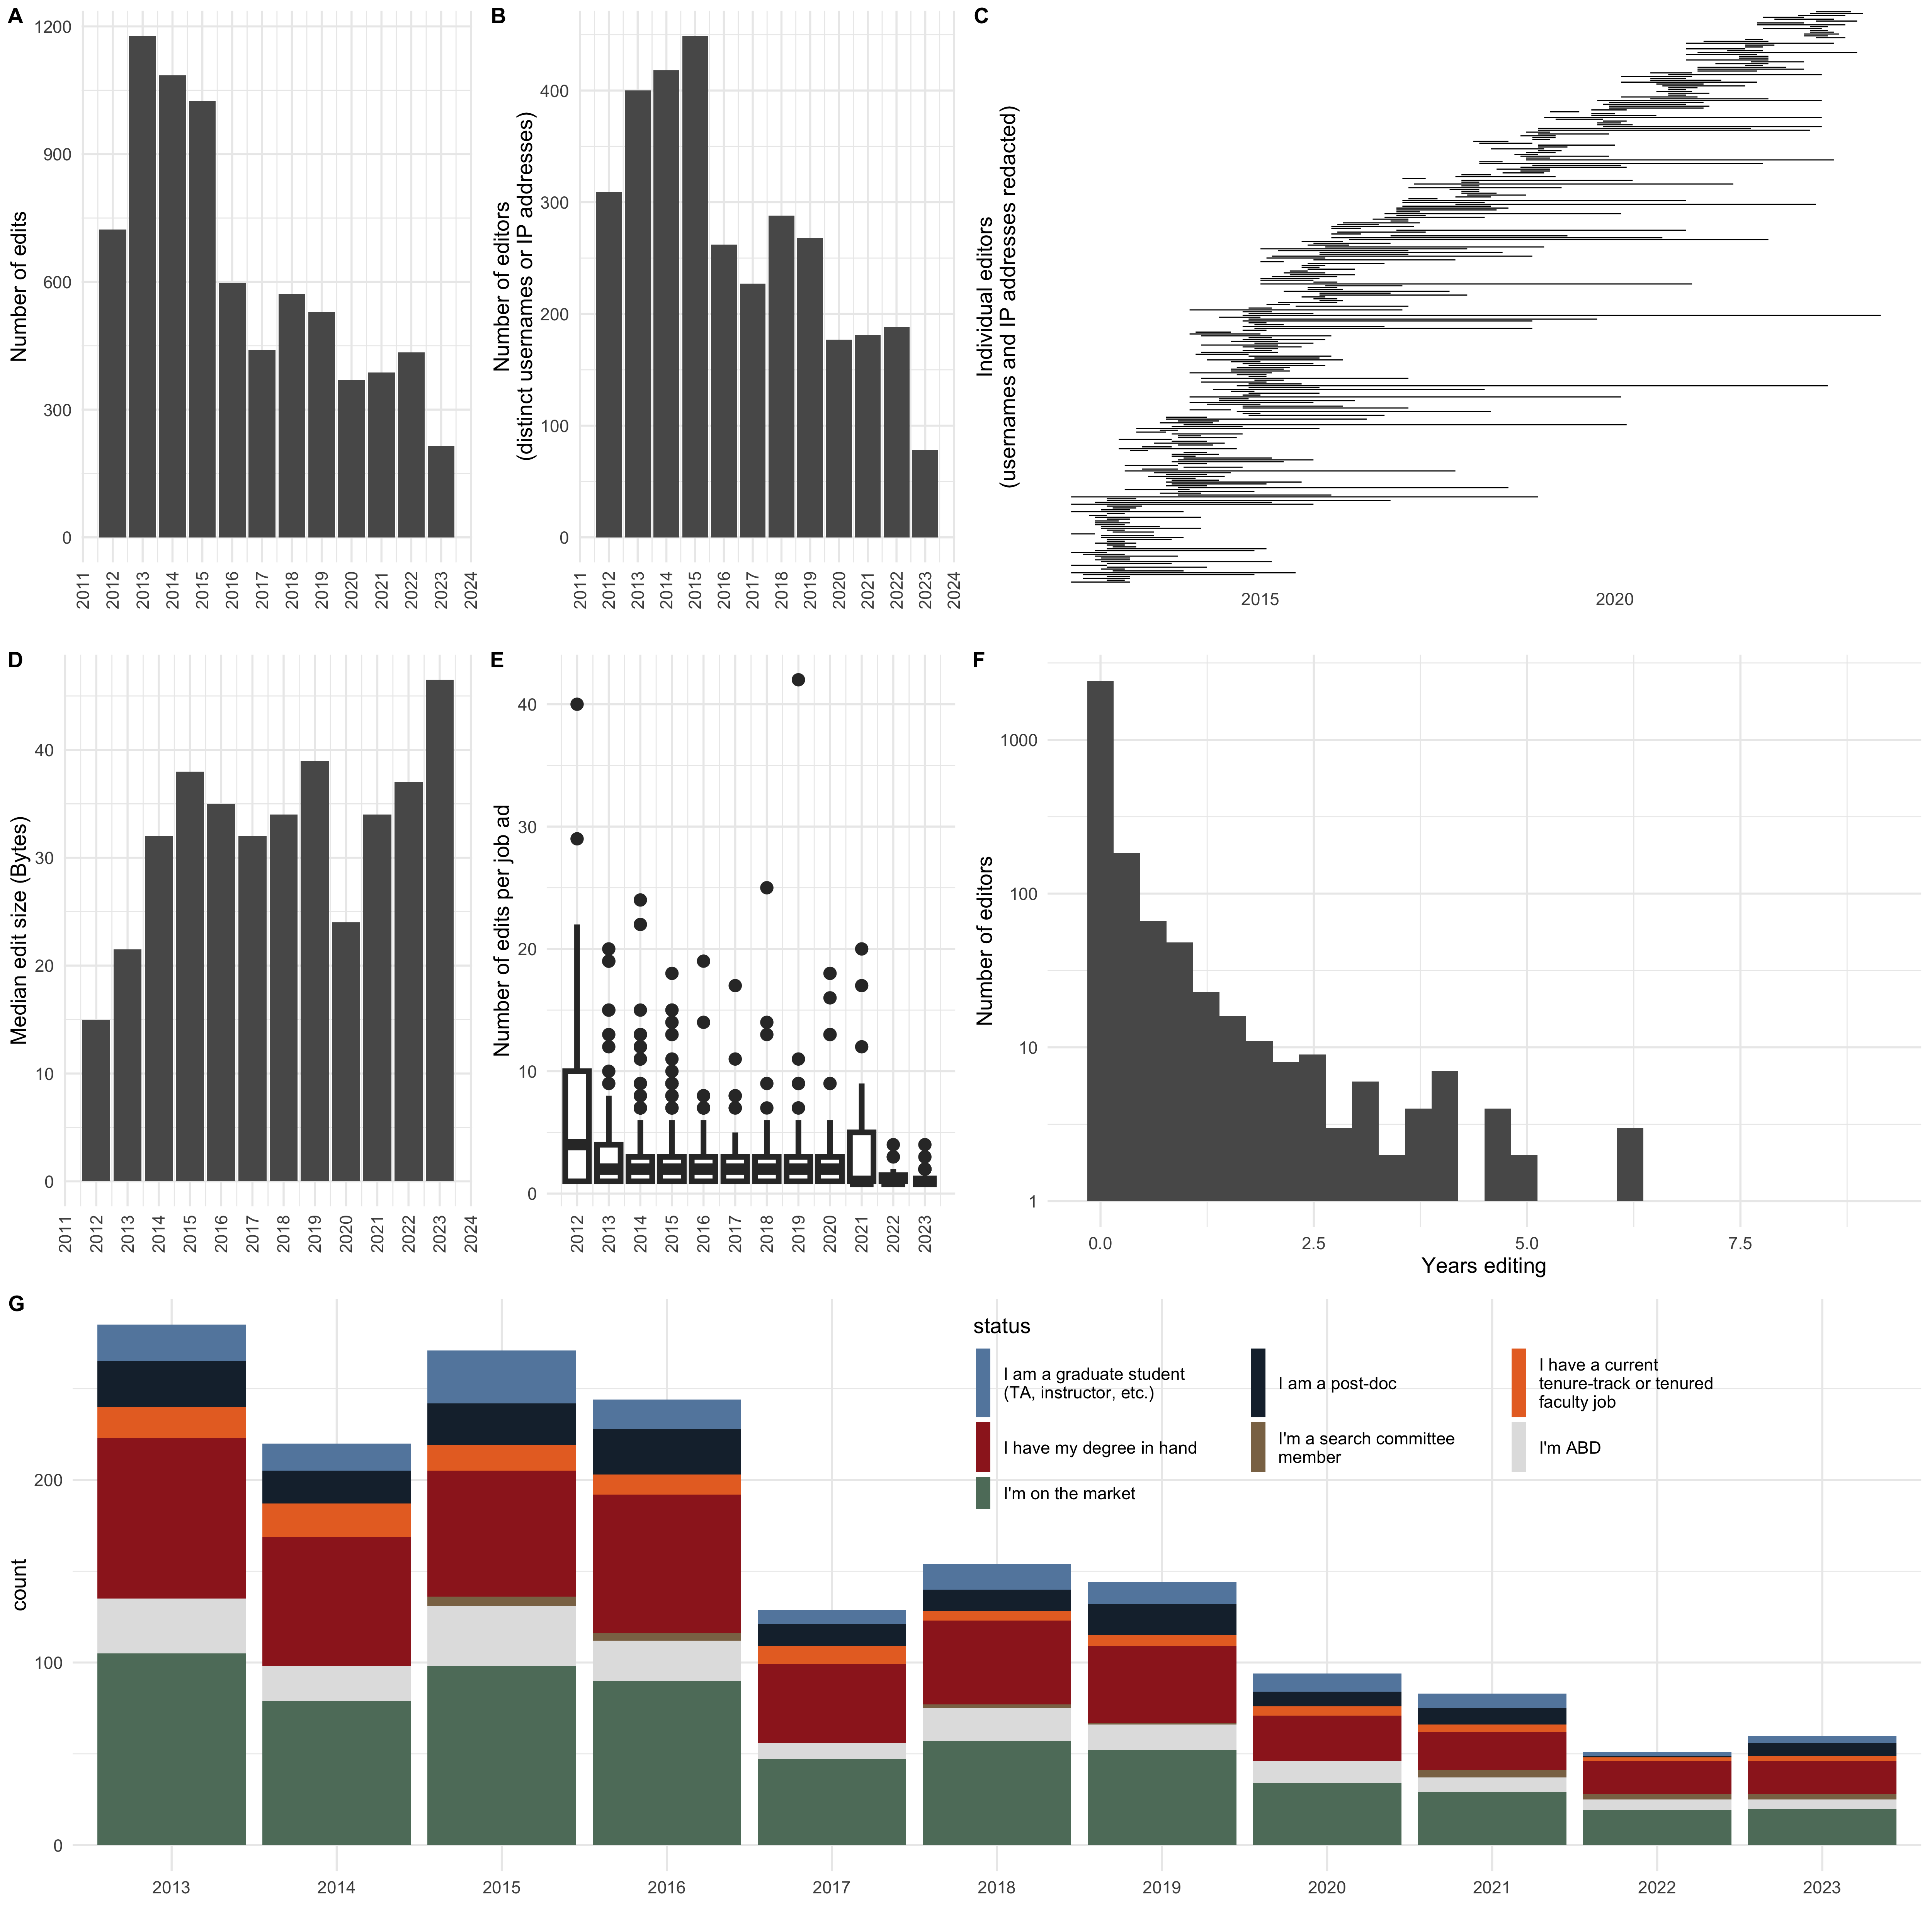
\includegraphics{article_files/figure-pdf/fig-panel-wiki-characteristics-1.pdf}

}

\caption{\label{fig-panel-wiki-characteristics}A: Total number of edits
to each Wiki page (additions and deletions) per year. B: Number of
unique editors, as represented by distinct usernames or IP addresses
(recorded for editors without usernames), active per year. C: Active
periods of individual editors, the black lines connect the date of the
first and last edit of all editors that were active for three months or
more. D: Typical size of each edit per year, either addition or removal
of text, one word is roughly 4-6 bytes. E: Distribution of the numbers
of edits per job ad for each year. F: Histogram showing that the
majority of editors are only active on the site for less than one year.
G: Breakdown of self-reported Wiki user categories for each year.}

\end{figure}%

Collaboratively-edited resources such as the Academic Jobs Wiki can be
highly variable in the amount and type of editorial activity over time.
It is important to characterise this activity to assess the reliability
of the content is as a source of information about the job market. The
MediaWiki technology used by Academic Jobs Wiki creates a public record
of every act of adding or removing text to any page in the Wiki (Barrett
2008). Figure~\ref{fig-panel-wiki-characteristics}, which allows us to
measure the dynamics of editing activity over the ten years of our study
period. Every edit includes the author's identity, recorded as either an
IP address (a numerical address that includes information about the
location of the user's computer) or a username. Of the 2824 unique
editors in our sample, 91\% used IP addresses rather than usernames, and
geolocation analysis shows that 81\% of IP addresses were based in the
U.S., indicating the Archaeology Jobs Wiki is primarily edited and
visited by users in the U.S. The number of edits and active editors
roughly halved from 2013 to 2017, and then continued to gradually
decline. Despite this downward trend, the size of individual edits
slightly increases over time, and the number of edits per job ad is
relatively constant across our study period. The majority of editors are
active on the site for a single day (n = 2241, 81\%). There are 412
(15\%) editors who were active for between one day and one year. Only
113 (n = 4\%) editors were active for more than one year, with 8 years
as the longest period any single editor was active on the Wiki. For
those active for more than one day, the average duration of editorial
activity is 4.6 years. This suggests that most of the editing activity
on the Wiki reflects a single season of job-searching. Editors with a
longer history likely come from two groups, job seekers participating in
multiple seasons of job applications, and faculty on search committees
posting multiple job ads. That said, inferring the number of editors
from the number of IP addresses is complicated by the high mobility of
job seekers. For example one person could be represented by several IP
addresses as they relocate from one city to another while working in a
series of short-term appointments such as post-doctoral fellowships and
adjunct teaching positions. This might result in an overestimation of
the number of editors on the Wiki and underestimation of the duration of
their editorial activity.

Longer-term editors who represent job seekers active for multiple
seasons reflect one of the underdiscussed realities of the academic job
market in archaeology---time spent on that market. Previous research on
professional trajectories in academic archaeology suggests that early
career researchers have a limited shelf life. Mackie and Rockwell, for
example, identify a hiring plateau that occurs around seven years after
candidates defend their PhDs (2023:5). However, too little time on the
market also seems to have a negative effect on placement rates---``very
few graduates obtain TT employment when they are all but dissertation
(ABD) or even immediately after graduation'' (Mackie and Rockwell
2023:5). These patterns are not restricted to the United States. In
Brami et al.'s (2023) survey of 419 early career researchers in European
archaeology, likelihood of holding a permanent position shifted relative
to time since PhD. Of the respondents who were one year or less than
four years post-PhD, only 3\% (3/116) held permanent positions. These
numbers increased slightly for participants who had been on the market
for five to seven years, with 14\% (7/49) holding permanent positions;
similarly, 18\% (6/34) of respondents who were on the market for eight
years or more held permanent positions.

This trajectory in archaeology---where there appears to be a temporal
``sweet spot'' post-PhD for obtaining permanent academic
positions---dovetails with a larger meta-analysis of the career
trajectories of PhDs from the humanities and humanistic social sciences.
Main et al. (2019) used longitudinal Graduate Education Survey (GES)
data from the Andrew W. Mellon Foundation to analyse the career
trajectories of over 5,000 PhDs from disciplines in the humanities and
humanistic social sciences at three time points: six months post-PhD,
three years post-PhD, and eight years post-PhD. The proportion of
surveyed doctorates in tenure-track or tenured faculty positions
increased with time since PhD---41\% of the sample held a tenure-track
position six months after defending, 64\% held a tenure-track position
three years after defending, and 68\% held a tenure-track or tenured
position eight years after defending. In keeping with broader patterns
observed across the humanities and social sciences, the variable tenures
of editors on the Archaeology Jobs Wiki may partially reflect the
temporal patterns in hiring relative to job seekers' time since PhD.

There seems to be a shift over time in the balance of editors who
identify as job-seekers versus search committee members, as indicated by
the number of self-reporting users over time. Panel G of
Figure~\ref{fig-panel-wiki-characteristics} shows the data found on each
page in a section labeled `current users', where users can volunteer to
update a table tracking the status of users. These data indicate that
the total number of self-reporting users, from the values recording at
`How many people use the wiki?', declined by 82\% during the study
period. At the same time, the proportion of users self-identifying as
``search committee members'' increased, from under 5\% in 2014--2018 to
over 14\% from 2020 onward. This suggests that, over time, fewer job
applicants have been contributing job postings and sharing information
about their experiences, and search committee members have increasingly
been posting job advertisements themselves. Overall, the Archaeology
Academic Jobs Wiki is best understood not as a comprehensive and neutral
archive of all jobs posted during the study period, but a biased sample
of the the jobs that early career applicants were most focused on
applying for, and sharing information about.

\subsection{Methods of data collection and
classification}\label{methods-of-data-collection-and-classification}

For each tenure-track job advertised on the Archaeology Academic Jobs
Wiki during 2013--2023, we read the text and recorded the name of the
hiring institution, the title of the position, and exact words and
phrases from the ad about the topical, geographic, and methodological
foci of the position into a Google form. The topical focus is what we
understood as the intellectual core of the position---examples of
topical foci included environmental archaeology, public archaeology, and
North American archaeology. The geographic focus is the region of the
world about which the ideal candidate has scholarly expertise, for
example, Southwest US, Mediterranean, or Asia and India. The methods
focus is the data-generating sub-field of archaeology mentioned in the
ad. Examples of methods used in this study include archaeobotany, lithic
analysis, and zooarchaeology. We also recorded the type and number of
documents requested in each ad (e.g.~cover letter, CV, statements on
research, teaching, diversity, syllabi, course descriptions, writing
samples, transcripts) and how many names/letters of recommenders were
requested in the ad.

After completing primary data collection, we studied the topical,
geographic, and methods text of each ad. Following the approach of Ryan
and Bernard (2003), we collaboratively and manually reduced the
variation in the raw data into 10--15 categories appearing in at least
20 (for topics and geography) or 10 (for methods) job ads to simplify
analysis and visualization. This means that some topics, such as gender
(mentioned in 6 ads) do not appear in our results because of their
rarity in the job ads. Full details of the category reduction, showing
the mapping between exact phrases found in the job ads and the
categories we used for our analysis, can be found in our Supplementary
Materials. Our final topic categories were: American archaeology,
Ancient Europe and Mediterranean, Archaeological science, Archaeological
theory, Bioarchaeology, Complex societies, Digital archaeology,
Environmental archaeology, Evolutionary anthropology, Indigenous and
historical archaeology, North Mesoamerican archaeology, Pleistocene
archaeology, and Public archaeology. Our geographic categories were:
Africa, Americas, Asia \& India, Canada \& Arctic, Europe,
Mediterranean, Meso- \& South America, Near East, Oceania, Midwest US,
Northeastern US, Southeast US, Southwest US, and Western US. Our methods
categories were: Archaeobotany, Archaeometry, Bioarchaeology, Ceramic
analysis, Computational and Digital archaeology, Geoarchaeology,
Landscape analysis, Lithic analysis, Material culture analysis, and
Zooarchaeology.

Individual ads could be recorded to have multiple or none of these
topical, geographic, and methods foci, and some of the foci overlap.
Some topics include geographic regions because this is how they are
typically understood by archaeologists. For example, Mesoamerican
archaeology is understood to refer to a specific time period \emph{and}
a specific geographic region. Similarly, we recorded digital archaeology
as both a method (when a job ad also had a clearly distinct topical
focus, such as historic archaeology) and a topic (when there were no
other topics mentioned in the job ad). While this polythetic approach
results in categorical overlaps that can make the data challenging to
interpret (Kuckartz 2014), in our view this reflects the complex
realities of how search committees express their needs when searching
for new faculty. Acknowledgement of overlaps also produces new insights
into hiring dynamics through revealing intersections between different
foci.

The entire R code (R Core Team 2024) and data files used for all the
analyses and visualizations contained in this paper are openly available
at https://doi.org/10.5281/zenodo.14798941 to enable re-use of materials
and improve reproducibility and transparency (Marwick 2017). All of the
figures, tables, and statistical test results presented here can be
independently reproduced with the code and data in this repository. The
code is released under the MIT license, the data as CC-0, and the
figures as CC-BY, to enable maximum re-use.

\section{Results}\label{results}

We collected data from 547 ads for tenure-track jobs in archaeology
posted during 2013--2023. We focus our analysis here on the 431 ads for
positions at U.S. universities. Figure~\ref{fig-show-basic-plots} shows
the count of ads for each year, where year refers to the year the job ad
was posted. Table~\ref{tbl-show-basic-counts} shows the breakdown by
different job types, ranks, and tenure status. Assistant Professor jobs
are consistently the most common title and rank of positions advertised,
while open rank or full professor are the least frequent. The ratio of
tenure-track to non-tenure-track positions is generally well above one;
in other words, this data set is dominated by tenure-track positions.
Only academic year 2013--2014 had more non-tenure-track positions than
tenure-track positions, which was followed by an upward trend peaking at
2018--2019 and then declining again into the present.

\begin{figure}

\centering{

\includegraphics[width=6.3in,height=\textheight]{../figures/fig-panel-per-year.png}

}

\caption{\label{fig-show-basic-plots}A: total number of job ads from US
institutions posted to the Academic Jobs Wiki for Archaeology in each
year, with coloured sections showing the proportion of jobs by title and
rank. B: Ratio of tenure-track to non-tenure-track positions over time.
The red line indicates a 1:1 ratio of tenure-track to non-tenure-track
positions, bars taller than that line indicate more tenure-track than
non-tenure-track positions in that year}

\end{figure}%

\global\setlength{\Oldarrayrulewidth}{\arrayrulewidth}

\global\setlength{\Oldtabcolsep}{\tabcolsep}

\setlength{\tabcolsep}{2pt}

\renewcommand*{\arraystretch}{1.5}



\providecommand{\ascline}[3]{\noalign{\global\arrayrulewidth #1}\arrayrulecolor[HTML]{#2}\cline{#3}}

\begin{longtable}[c]{|p{0.84in}|p{1.02in}|p{1.05in}|p{0.78in}|p{0.68in}|p{1.45in}|p{0.30in}|p{0.37in}}

\caption{\label{tbl-show-basic-counts}Breakdown of counts of job ads by
rank and tenure status. Values in parentheses are for the United States
only. TT = tenure-track, US-only, NTT = non-tenure-track, US and
elsewhere. Not all ads include unambiguous information about tenure
status, so the sum of TT and NTT does not equal the sum of all jobs in
all ranks.}

\tabularnewline

\ascline{1.5pt}{666666}{1-8}

\multicolumn{1}{>{\centering}m{\dimexpr 0.84in+0\tabcolsep}}{\textcolor[HTML]{000000}{\fontsize{7}{7}\selectfont{\global\setmainfont{Helvetica}{Year\ ad\ posted}}}} & \multicolumn{1}{>{\centering}m{\dimexpr 1.02in+0\tabcolsep}}{\textcolor[HTML]{000000}{\fontsize{7}{7}\selectfont{\global\setmainfont{Helvetica}{Assistant\ Professor}}}} & \multicolumn{1}{>{\centering}m{\dimexpr 1.05in+0\tabcolsep}}{\textcolor[HTML]{000000}{\fontsize{7}{7}\selectfont{\global\setmainfont{Helvetica}{Associate\ Professor}}}} & \multicolumn{1}{>{\centering}m{\dimexpr 0.78in+0\tabcolsep}}{\textcolor[HTML]{000000}{\fontsize{7}{7}\selectfont{\global\setmainfont{Helvetica}{Full\ Professor}}}} & \multicolumn{1}{>{\centering}m{\dimexpr 0.68in+0\tabcolsep}}{\textcolor[HTML]{000000}{\fontsize{7}{7}\selectfont{\global\setmainfont{Helvetica}{Open\ Rank}}}} & \multicolumn{1}{>{\centering}m{\dimexpr 1.45in+0\tabcolsep}}{\textcolor[HTML]{000000}{\fontsize{7}{7}\selectfont{\global\setmainfont{Helvetica}{Other\ (Curator,\ Director,\ etc.)}}}} & \multicolumn{1}{>{\centering}m{\dimexpr 0.3in+0\tabcolsep}}{\textcolor[HTML]{000000}{\fontsize{7}{7}\selectfont{\global\setmainfont{Helvetica}{TT}}}} & \multicolumn{1}{>{\centering}m{\dimexpr 0.37in+0\tabcolsep}}{\textcolor[HTML]{000000}{\fontsize{7}{7}\selectfont{\global\setmainfont{Helvetica}{NTT}}}} \\

\ascline{1.5pt}{666666}{1-8}\endfirsthead 

\ascline{1.5pt}{666666}{1-8}

\multicolumn{1}{>{\centering}m{\dimexpr 0.84in+0\tabcolsep}}{\textcolor[HTML]{000000}{\fontsize{7}{7}\selectfont{\global\setmainfont{Helvetica}{Year\ ad\ posted}}}} & \multicolumn{1}{>{\centering}m{\dimexpr 1.02in+0\tabcolsep}}{\textcolor[HTML]{000000}{\fontsize{7}{7}\selectfont{\global\setmainfont{Helvetica}{Assistant\ Professor}}}} & \multicolumn{1}{>{\centering}m{\dimexpr 1.05in+0\tabcolsep}}{\textcolor[HTML]{000000}{\fontsize{7}{7}\selectfont{\global\setmainfont{Helvetica}{Associate\ Professor}}}} & \multicolumn{1}{>{\centering}m{\dimexpr 0.78in+0\tabcolsep}}{\textcolor[HTML]{000000}{\fontsize{7}{7}\selectfont{\global\setmainfont{Helvetica}{Full\ Professor}}}} & \multicolumn{1}{>{\centering}m{\dimexpr 0.68in+0\tabcolsep}}{\textcolor[HTML]{000000}{\fontsize{7}{7}\selectfont{\global\setmainfont{Helvetica}{Open\ Rank}}}} & \multicolumn{1}{>{\centering}m{\dimexpr 1.45in+0\tabcolsep}}{\textcolor[HTML]{000000}{\fontsize{7}{7}\selectfont{\global\setmainfont{Helvetica}{Other\ (Curator,\ Director,\ etc.)}}}} & \multicolumn{1}{>{\centering}m{\dimexpr 0.3in+0\tabcolsep}}{\textcolor[HTML]{000000}{\fontsize{7}{7}\selectfont{\global\setmainfont{Helvetica}{TT}}}} & \multicolumn{1}{>{\centering}m{\dimexpr 0.37in+0\tabcolsep}}{\textcolor[HTML]{000000}{\fontsize{7}{7}\selectfont{\global\setmainfont{Helvetica}{NTT}}}} \\

\ascline{1.5pt}{666666}{1-8}\endhead



\multicolumn{1}{>{\centering}m{\dimexpr 0.84in+0\tabcolsep}}{\textcolor[HTML]{000000}{\fontsize{7}{7}\selectfont{\global\setmainfont{Helvetica}{2012-2013}}}} & \multicolumn{1}{>{\centering}m{\dimexpr 1.02in+0\tabcolsep}}{\textcolor[HTML]{000000}{\fontsize{7}{7}\selectfont{\global\setmainfont{Helvetica}{27\ (26)}}}} & \multicolumn{1}{>{\centering}m{\dimexpr 1.05in+0\tabcolsep}}{\textcolor[HTML]{000000}{\fontsize{7}{7}\selectfont{\global\setmainfont{Helvetica}{7\ (7)}}}} & \multicolumn{1}{>{\centering}m{\dimexpr 0.78in+0\tabcolsep}}{\textcolor[HTML]{000000}{\fontsize{7}{7}\selectfont{\global\setmainfont{Helvetica}{-\ (-)}}}} & \multicolumn{1}{>{\centering}m{\dimexpr 0.68in+0\tabcolsep}}{\textcolor[HTML]{000000}{\fontsize{7}{7}\selectfont{\global\setmainfont{Helvetica}{4\ (4)}}}} & \multicolumn{1}{>{\centering}m{\dimexpr 1.45in+0\tabcolsep}}{\textcolor[HTML]{000000}{\fontsize{7}{7}\selectfont{\global\setmainfont{Helvetica}{4\ (4)}}}} & \multicolumn{1}{>{\centering}m{\dimexpr 0.3in+0\tabcolsep}}{\textcolor[HTML]{000000}{\fontsize{7}{7}\selectfont{\global\setmainfont{Helvetica}{41}}}} & \multicolumn{1}{>{\centering}m{\dimexpr 0.37in+0\tabcolsep}}{\textcolor[HTML]{000000}{\fontsize{7}{7}\selectfont{\global\setmainfont{Helvetica}{24}}}} \\





\multicolumn{1}{>{\centering}m{\dimexpr 0.84in+0\tabcolsep}}{\textcolor[HTML]{000000}{\fontsize{7}{7}\selectfont{\global\setmainfont{Helvetica}{2013-2014}}}} & \multicolumn{1}{>{\centering}m{\dimexpr 1.02in+0\tabcolsep}}{\textcolor[HTML]{000000}{\fontsize{7}{7}\selectfont{\global\setmainfont{Helvetica}{19\ (14)}}}} & \multicolumn{1}{>{\centering}m{\dimexpr 1.05in+0\tabcolsep}}{\textcolor[HTML]{000000}{\fontsize{7}{7}\selectfont{\global\setmainfont{Helvetica}{5\ (2)}}}} & \multicolumn{1}{>{\centering}m{\dimexpr 0.78in+0\tabcolsep}}{\textcolor[HTML]{000000}{\fontsize{7}{7}\selectfont{\global\setmainfont{Helvetica}{3\ (3)}}}} & \multicolumn{1}{>{\centering}m{\dimexpr 0.68in+0\tabcolsep}}{\textcolor[HTML]{000000}{\fontsize{7}{7}\selectfont{\global\setmainfont{Helvetica}{2\ (1)}}}} & \multicolumn{1}{>{\centering}m{\dimexpr 1.45in+0\tabcolsep}}{\textcolor[HTML]{000000}{\fontsize{7}{7}\selectfont{\global\setmainfont{Helvetica}{5\ (1)}}}} & \multicolumn{1}{>{\centering}m{\dimexpr 0.3in+0\tabcolsep}}{\textcolor[HTML]{000000}{\fontsize{7}{7}\selectfont{\global\setmainfont{Helvetica}{21}}}} & \multicolumn{1}{>{\centering}m{\dimexpr 0.37in+0\tabcolsep}}{\textcolor[HTML]{000000}{\fontsize{7}{7}\selectfont{\global\setmainfont{Helvetica}{77}}}} \\





\multicolumn{1}{>{\centering}m{\dimexpr 0.84in+0\tabcolsep}}{\textcolor[HTML]{000000}{\fontsize{7}{7}\selectfont{\global\setmainfont{Helvetica}{2014-2015}}}} & \multicolumn{1}{>{\centering}m{\dimexpr 1.02in+0\tabcolsep}}{\textcolor[HTML]{000000}{\fontsize{7}{7}\selectfont{\global\setmainfont{Helvetica}{42\ (36)}}}} & \multicolumn{1}{>{\centering}m{\dimexpr 1.05in+0\tabcolsep}}{\textcolor[HTML]{000000}{\fontsize{7}{7}\selectfont{\global\setmainfont{Helvetica}{6\ (6)}}}} & \multicolumn{1}{>{\centering}m{\dimexpr 0.78in+0\tabcolsep}}{\textcolor[HTML]{000000}{\fontsize{7}{7}\selectfont{\global\setmainfont{Helvetica}{3\ (3)}}}} & \multicolumn{1}{>{\centering}m{\dimexpr 0.68in+0\tabcolsep}}{\textcolor[HTML]{000000}{\fontsize{7}{7}\selectfont{\global\setmainfont{Helvetica}{9\ (8)}}}} & \multicolumn{1}{>{\centering}m{\dimexpr 1.45in+0\tabcolsep}}{\textcolor[HTML]{000000}{\fontsize{7}{7}\selectfont{\global\setmainfont{Helvetica}{5\ (4)}}}} & \multicolumn{1}{>{\centering}m{\dimexpr 0.3in+0\tabcolsep}}{\textcolor[HTML]{000000}{\fontsize{7}{7}\selectfont{\global\setmainfont{Helvetica}{57}}}} & \multicolumn{1}{>{\centering}m{\dimexpr 0.37in+0\tabcolsep}}{\textcolor[HTML]{000000}{\fontsize{7}{7}\selectfont{\global\setmainfont{Helvetica}{35}}}} \\





\multicolumn{1}{>{\centering}m{\dimexpr 0.84in+0\tabcolsep}}{\textcolor[HTML]{000000}{\fontsize{7}{7}\selectfont{\global\setmainfont{Helvetica}{2015-2016}}}} & \multicolumn{1}{>{\centering}m{\dimexpr 1.02in+0\tabcolsep}}{\textcolor[HTML]{000000}{\fontsize{7}{7}\selectfont{\global\setmainfont{Helvetica}{44\ (39)}}}} & \multicolumn{1}{>{\centering}m{\dimexpr 1.05in+0\tabcolsep}}{\textcolor[HTML]{000000}{\fontsize{7}{7}\selectfont{\global\setmainfont{Helvetica}{5\ (4)}}}} & \multicolumn{1}{>{\centering}m{\dimexpr 0.78in+0\tabcolsep}}{\textcolor[HTML]{000000}{\fontsize{7}{7}\selectfont{\global\setmainfont{Helvetica}{1\ (1)}}}} & \multicolumn{1}{>{\centering}m{\dimexpr 0.68in+0\tabcolsep}}{\textcolor[HTML]{000000}{\fontsize{7}{7}\selectfont{\global\setmainfont{Helvetica}{2\ (2)}}}} & \multicolumn{1}{>{\centering}m{\dimexpr 1.45in+0\tabcolsep}}{\textcolor[HTML]{000000}{\fontsize{7}{7}\selectfont{\global\setmainfont{Helvetica}{5\ (3)}}}} & \multicolumn{1}{>{\centering}m{\dimexpr 0.3in+0\tabcolsep}}{\textcolor[HTML]{000000}{\fontsize{7}{7}\selectfont{\global\setmainfont{Helvetica}{49}}}} & \multicolumn{1}{>{\centering}m{\dimexpr 0.37in+0\tabcolsep}}{\textcolor[HTML]{000000}{\fontsize{7}{7}\selectfont{\global\setmainfont{Helvetica}{25}}}} \\





\multicolumn{1}{>{\centering}m{\dimexpr 0.84in+0\tabcolsep}}{\textcolor[HTML]{000000}{\fontsize{7}{7}\selectfont{\global\setmainfont{Helvetica}{2016-2017}}}} & \multicolumn{1}{>{\centering}m{\dimexpr 1.02in+0\tabcolsep}}{\textcolor[HTML]{000000}{\fontsize{7}{7}\selectfont{\global\setmainfont{Helvetica}{35\ (27)}}}} & \multicolumn{1}{>{\centering}m{\dimexpr 1.05in+0\tabcolsep}}{\textcolor[HTML]{000000}{\fontsize{7}{7}\selectfont{\global\setmainfont{Helvetica}{4\ (4)}}}} & \multicolumn{1}{>{\centering}m{\dimexpr 0.78in+0\tabcolsep}}{\textcolor[HTML]{000000}{\fontsize{7}{7}\selectfont{\global\setmainfont{Helvetica}{1\ (1)}}}} & \multicolumn{1}{>{\centering}m{\dimexpr 0.68in+0\tabcolsep}}{\textcolor[HTML]{000000}{\fontsize{7}{7}\selectfont{\global\setmainfont{Helvetica}{2\ (2)}}}} & \multicolumn{1}{>{\centering}m{\dimexpr 1.45in+0\tabcolsep}}{\textcolor[HTML]{000000}{\fontsize{7}{7}\selectfont{\global\setmainfont{Helvetica}{-\ (-)}}}} & \multicolumn{1}{>{\centering}m{\dimexpr 0.3in+0\tabcolsep}}{\textcolor[HTML]{000000}{\fontsize{7}{7}\selectfont{\global\setmainfont{Helvetica}{34}}}} & \multicolumn{1}{>{\centering}m{\dimexpr 0.37in+0\tabcolsep}}{\textcolor[HTML]{000000}{\fontsize{7}{7}\selectfont{\global\setmainfont{Helvetica}{25}}}} \\





\multicolumn{1}{>{\centering}m{\dimexpr 0.84in+0\tabcolsep}}{\textcolor[HTML]{000000}{\fontsize{7}{7}\selectfont{\global\setmainfont{Helvetica}{2017-2018}}}} & \multicolumn{1}{>{\centering}m{\dimexpr 1.02in+0\tabcolsep}}{\textcolor[HTML]{000000}{\fontsize{7}{7}\selectfont{\global\setmainfont{Helvetica}{30\ (25)}}}} & \multicolumn{1}{>{\centering}m{\dimexpr 1.05in+0\tabcolsep}}{\textcolor[HTML]{000000}{\fontsize{7}{7}\selectfont{\global\setmainfont{Helvetica}{7\ (7)}}}} & \multicolumn{1}{>{\centering}m{\dimexpr 0.78in+0\tabcolsep}}{\textcolor[HTML]{000000}{\fontsize{7}{7}\selectfont{\global\setmainfont{Helvetica}{-\ (-)}}}} & \multicolumn{1}{>{\centering}m{\dimexpr 0.68in+0\tabcolsep}}{\textcolor[HTML]{000000}{\fontsize{7}{7}\selectfont{\global\setmainfont{Helvetica}{3\ (3)}}}} & \multicolumn{1}{>{\centering}m{\dimexpr 1.45in+0\tabcolsep}}{\textcolor[HTML]{000000}{\fontsize{7}{7}\selectfont{\global\setmainfont{Helvetica}{8\ (6)}}}} & \multicolumn{1}{>{\centering}m{\dimexpr 0.3in+0\tabcolsep}}{\textcolor[HTML]{000000}{\fontsize{7}{7}\selectfont{\global\setmainfont{Helvetica}{41}}}} & \multicolumn{1}{>{\centering}m{\dimexpr 0.37in+0\tabcolsep}}{\textcolor[HTML]{000000}{\fontsize{7}{7}\selectfont{\global\setmainfont{Helvetica}{20}}}} \\





\multicolumn{1}{>{\centering}m{\dimexpr 0.84in+0\tabcolsep}}{\textcolor[HTML]{000000}{\fontsize{7}{7}\selectfont{\global\setmainfont{Helvetica}{2018-2019}}}} & \multicolumn{1}{>{\centering}m{\dimexpr 1.02in+0\tabcolsep}}{\textcolor[HTML]{000000}{\fontsize{7}{7}\selectfont{\global\setmainfont{Helvetica}{35\ (33)}}}} & \multicolumn{1}{>{\centering}m{\dimexpr 1.05in+0\tabcolsep}}{\textcolor[HTML]{000000}{\fontsize{7}{7}\selectfont{\global\setmainfont{Helvetica}{5\ (4)}}}} & \multicolumn{1}{>{\centering}m{\dimexpr 0.78in+0\tabcolsep}}{\textcolor[HTML]{000000}{\fontsize{7}{7}\selectfont{\global\setmainfont{Helvetica}{1\ (1)}}}} & \multicolumn{1}{>{\centering}m{\dimexpr 0.68in+0\tabcolsep}}{\textcolor[HTML]{000000}{\fontsize{7}{7}\selectfont{\global\setmainfont{Helvetica}{1\ (1)}}}} & \multicolumn{1}{>{\centering}m{\dimexpr 1.45in+0\tabcolsep}}{\textcolor[HTML]{000000}{\fontsize{7}{7}\selectfont{\global\setmainfont{Helvetica}{5\ (4)}}}} & \multicolumn{1}{>{\centering}m{\dimexpr 0.3in+0\tabcolsep}}{\textcolor[HTML]{000000}{\fontsize{7}{7}\selectfont{\global\setmainfont{Helvetica}{43}}}} & \multicolumn{1}{>{\centering}m{\dimexpr 0.37in+0\tabcolsep}}{\textcolor[HTML]{000000}{\fontsize{7}{7}\selectfont{\global\setmainfont{Helvetica}{14}}}} \\





\multicolumn{1}{>{\centering}m{\dimexpr 0.84in+0\tabcolsep}}{\textcolor[HTML]{000000}{\fontsize{7}{7}\selectfont{\global\setmainfont{Helvetica}{2019-2020}}}} & \multicolumn{1}{>{\centering}m{\dimexpr 1.02in+0\tabcolsep}}{\textcolor[HTML]{000000}{\fontsize{7}{7}\selectfont{\global\setmainfont{Helvetica}{33\ (29)}}}} & \multicolumn{1}{>{\centering}m{\dimexpr 1.05in+0\tabcolsep}}{\textcolor[HTML]{000000}{\fontsize{7}{7}\selectfont{\global\setmainfont{Helvetica}{2\ (2)}}}} & \multicolumn{1}{>{\centering}m{\dimexpr 0.78in+0\tabcolsep}}{\textcolor[HTML]{000000}{\fontsize{7}{7}\selectfont{\global\setmainfont{Helvetica}{1\ (-)}}}} & \multicolumn{1}{>{\centering}m{\dimexpr 0.68in+0\tabcolsep}}{\textcolor[HTML]{000000}{\fontsize{7}{7}\selectfont{\global\setmainfont{Helvetica}{3\ (3)}}}} & \multicolumn{1}{>{\centering}m{\dimexpr 1.45in+0\tabcolsep}}{\textcolor[HTML]{000000}{\fontsize{7}{7}\selectfont{\global\setmainfont{Helvetica}{2\ (1)}}}} & \multicolumn{1}{>{\centering}m{\dimexpr 0.3in+0\tabcolsep}}{\textcolor[HTML]{000000}{\fontsize{7}{7}\selectfont{\global\setmainfont{Helvetica}{34}}}} & \multicolumn{1}{>{\centering}m{\dimexpr 0.37in+0\tabcolsep}}{\textcolor[HTML]{000000}{\fontsize{7}{7}\selectfont{\global\setmainfont{Helvetica}{20}}}} \\





\multicolumn{1}{>{\centering}m{\dimexpr 0.84in+0\tabcolsep}}{\textcolor[HTML]{000000}{\fontsize{7}{7}\selectfont{\global\setmainfont{Helvetica}{2020-2021}}}} & \multicolumn{1}{>{\centering}m{\dimexpr 1.02in+0\tabcolsep}}{\textcolor[HTML]{000000}{\fontsize{7}{7}\selectfont{\global\setmainfont{Helvetica}{14\ (11)}}}} & \multicolumn{1}{>{\centering}m{\dimexpr 1.05in+0\tabcolsep}}{\textcolor[HTML]{000000}{\fontsize{7}{7}\selectfont{\global\setmainfont{Helvetica}{3\ (-)}}}} & \multicolumn{1}{>{\centering}m{\dimexpr 0.78in+0\tabcolsep}}{\textcolor[HTML]{000000}{\fontsize{7}{7}\selectfont{\global\setmainfont{Helvetica}{1\ (1)}}}} & \multicolumn{1}{>{\centering}m{\dimexpr 0.68in+0\tabcolsep}}{\textcolor[HTML]{000000}{\fontsize{7}{7}\selectfont{\global\setmainfont{Helvetica}{-\ (-)}}}} & \multicolumn{1}{>{\centering}m{\dimexpr 1.45in+0\tabcolsep}}{\textcolor[HTML]{000000}{\fontsize{7}{7}\selectfont{\global\setmainfont{Helvetica}{2\ (-)}}}} & \multicolumn{1}{>{\centering}m{\dimexpr 0.3in+0\tabcolsep}}{\textcolor[HTML]{000000}{\fontsize{7}{7}\selectfont{\global\setmainfont{Helvetica}{12}}}} & \multicolumn{1}{>{\centering}m{\dimexpr 0.37in+0\tabcolsep}}{\textcolor[HTML]{000000}{\fontsize{7}{7}\selectfont{\global\setmainfont{Helvetica}{19}}}} \\





\multicolumn{1}{>{\centering}m{\dimexpr 0.84in+0\tabcolsep}}{\textcolor[HTML]{000000}{\fontsize{7}{7}\selectfont{\global\setmainfont{Helvetica}{2021-2022}}}} & \multicolumn{1}{>{\centering}m{\dimexpr 1.02in+0\tabcolsep}}{\textcolor[HTML]{000000}{\fontsize{7}{7}\selectfont{\global\setmainfont{Helvetica}{33\ (29)}}}} & \multicolumn{1}{>{\centering}m{\dimexpr 1.05in+0\tabcolsep}}{\textcolor[HTML]{000000}{\fontsize{7}{7}\selectfont{\global\setmainfont{Helvetica}{2\ (1)}}}} & \multicolumn{1}{>{\centering}m{\dimexpr 0.78in+0\tabcolsep}}{\textcolor[HTML]{000000}{\fontsize{7}{7}\selectfont{\global\setmainfont{Helvetica}{2\ (2)}}}} & \multicolumn{1}{>{\centering}m{\dimexpr 0.68in+0\tabcolsep}}{\textcolor[HTML]{000000}{\fontsize{7}{7}\selectfont{\global\setmainfont{Helvetica}{5\ (2)}}}} & \multicolumn{1}{>{\centering}m{\dimexpr 1.45in+0\tabcolsep}}{\textcolor[HTML]{000000}{\fontsize{7}{7}\selectfont{\global\setmainfont{Helvetica}{8\ (5)}}}} & \multicolumn{1}{>{\centering}m{\dimexpr 0.3in+0\tabcolsep}}{\textcolor[HTML]{000000}{\fontsize{7}{7}\selectfont{\global\setmainfont{Helvetica}{39}}}} & \multicolumn{1}{>{\centering}m{\dimexpr 0.37in+0\tabcolsep}}{\textcolor[HTML]{000000}{\fontsize{7}{7}\selectfont{\global\setmainfont{Helvetica}{27}}}} \\





\multicolumn{1}{>{\centering}m{\dimexpr 0.84in+0\tabcolsep}}{\textcolor[HTML]{000000}{\fontsize{7}{7}\selectfont{\global\setmainfont{Helvetica}{2022-2023}}}} & \multicolumn{1}{>{\centering}m{\dimexpr 1.02in+0\tabcolsep}}{\textcolor[HTML]{000000}{\fontsize{7}{7}\selectfont{\global\setmainfont{Helvetica}{67\ (41)}}}} & \multicolumn{1}{>{\centering}m{\dimexpr 1.05in+0\tabcolsep}}{\textcolor[HTML]{000000}{\fontsize{7}{7}\selectfont{\global\setmainfont{Helvetica}{10\ (8)}}}} & \multicolumn{1}{>{\centering}m{\dimexpr 0.78in+0\tabcolsep}}{\textcolor[HTML]{000000}{\fontsize{7}{7}\selectfont{\global\setmainfont{Helvetica}{4\ (4)}}}} & \multicolumn{1}{>{\centering}m{\dimexpr 0.68in+0\tabcolsep}}{\textcolor[HTML]{000000}{\fontsize{7}{7}\selectfont{\global\setmainfont{Helvetica}{1\ (-)}}}} & \multicolumn{1}{>{\centering}m{\dimexpr 1.45in+0\tabcolsep}}{\textcolor[HTML]{000000}{\fontsize{7}{7}\selectfont{\global\setmainfont{Helvetica}{19\ (6)}}}} & \multicolumn{1}{>{\centering}m{\dimexpr 0.3in+0\tabcolsep}}{\textcolor[HTML]{000000}{\fontsize{7}{7}\selectfont{\global\setmainfont{Helvetica}{59}}}} & \multicolumn{1}{>{\centering}m{\dimexpr 0.37in+0\tabcolsep}}{\textcolor[HTML]{000000}{\fontsize{7}{7}\selectfont{\global\setmainfont{Helvetica}{126}}}} \\

\ascline{1.5pt}{666666}{1-8}


\end{longtable}

\arrayrulecolor[HTML]{000000}

\global\setlength{\arrayrulewidth}{\Oldarrayrulewidth}

\global\setlength{\tabcolsep}{\Oldtabcolsep}

\renewcommand*{\arraystretch}{1}

\subsection{Characteristics of the hiring
institutions}\label{characteristics-of-the-hiring-institutions}

\begin{figure}

\centering{

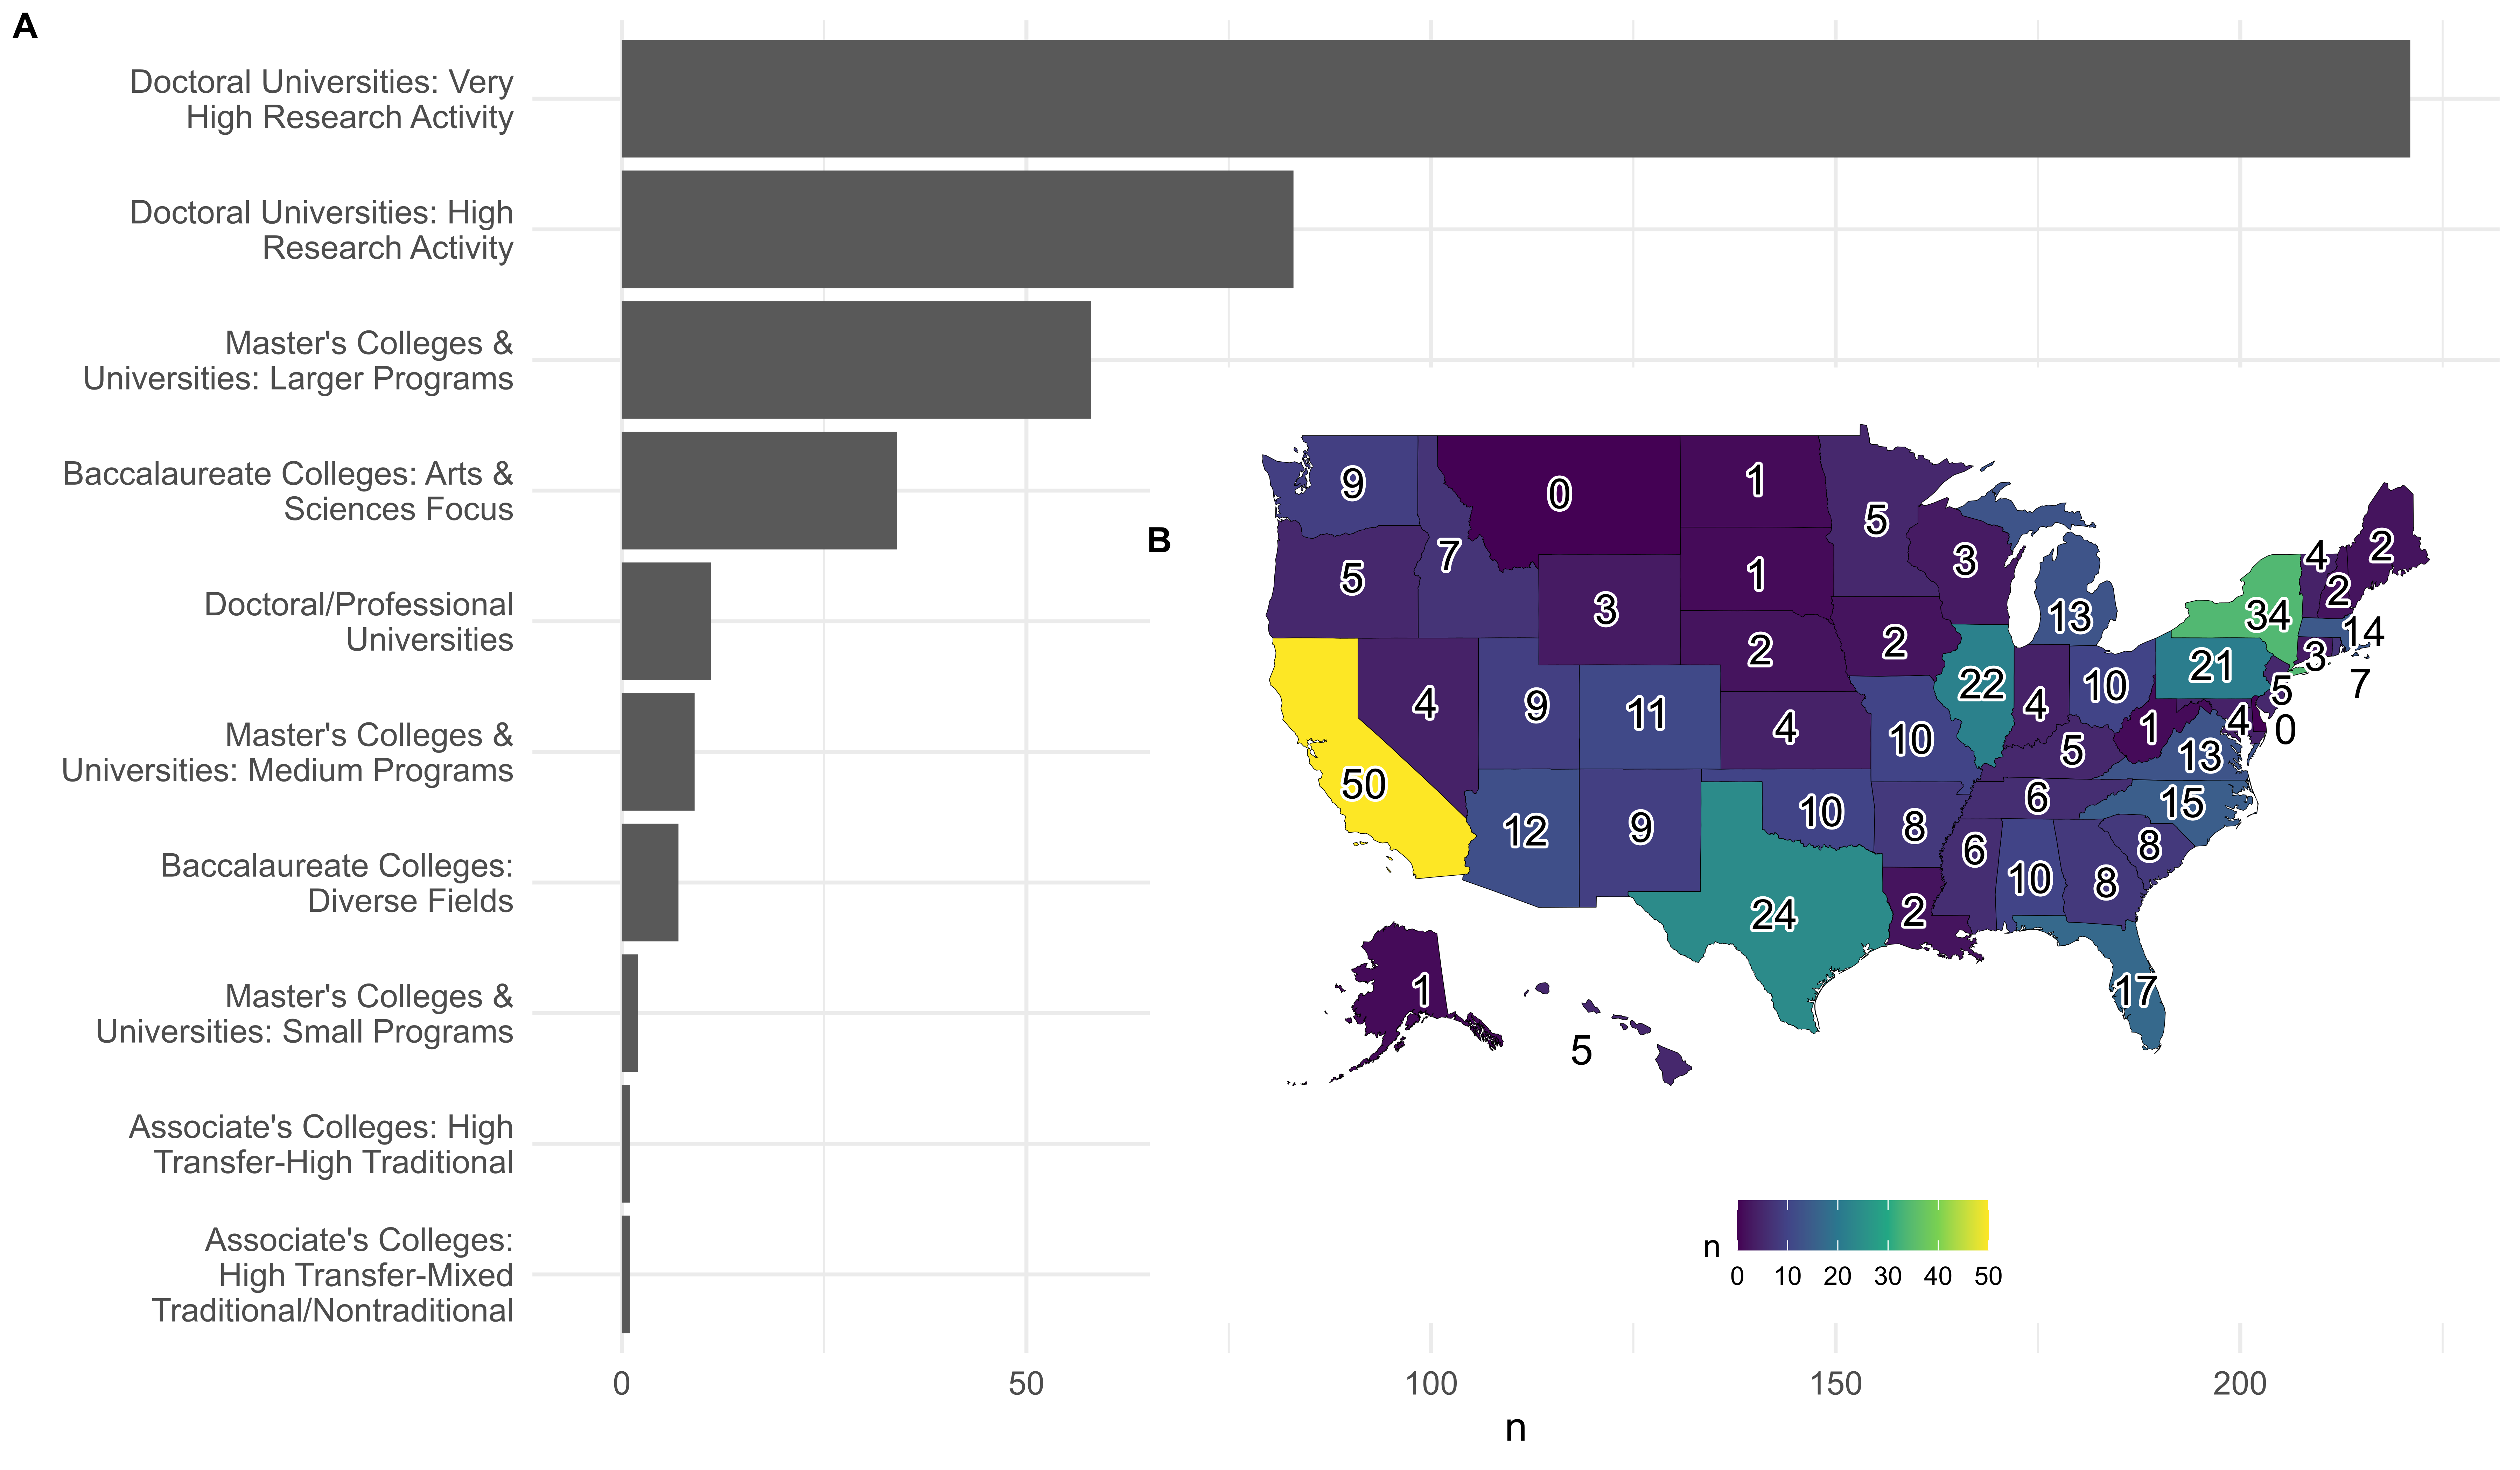
\includegraphics[width=7.2in,height=\textheight]{../figures/fig-map-and-carnegie-classification-hand-edit.png}

}

\caption{\label{fig-show-map-of-hiring-institution-and-cc}A: Frequency
of hiring institution by Carnegie classification. B: Inset shows map of
the United States showing the count of tenure-track job ads posted by
all institutions in each state during 2013 -- 2023}

\end{figure}%

Panel A of Figure~\ref{fig-show-map-of-hiring-institution-and-cc} shows
the frequencies of hiring institutions according to their Carnegie
Classification, a framework for classifying U.S. colleges and
universities according to the types of degrees awarded, levels of
research activity, and topical foci (Shulman 2001). Doctoral
universities with high and very high research activity are by far the
most active institutions hiring archaeology faculty. Associate's
colleges, also known as community colleges, rarely post job ads for
archaeology faculty.

The geographic distribution of hiring institutions is shown in
Figure~\ref{fig-show-map-of-hiring-institution-and-cc} Panel B.
California posted almost twice as many job ads as the next most active
states. After California, the states that posted the most ads during
2013--2023 include New York, Texas, Pennsylvania, and Florida. These top
five states correspond to the top five most populous U.S. states,
suggesting that rates of hiring are approximately proportional to
population density. The top five states for job ads are also the five
states with highest number of degrees awarded in Anthropology (National
Center for Education Statistics 2025). Similarly, the lowest counts of
job ads were observed in states with the lowest populations: North
Dakota, South Dakota, Alaska, and Nebraska. No institutions in Montana
posted a job ad during this period. The implication here is that
job-seekers who are able to relocate to populous areas will have more
employment options.

\subsection{Geographic trends in job ads over
time}\label{geographic-trends-in-job-ads-over-time}

\begin{figure}

\centering{

\includegraphics[width=7.2in,height=\textheight]{../figures/fig-geo-focus-by-year.png}

}

\caption{\label{fig-show-geo-trends}A: Frequency of locations mentioned
in the text of the job ads. B: Popularity of locations in job ads over
time for locations that appear in 20 or more ads. Individual data points
are shown, overlain by a locally weighted regression line for each
location to indicate temporal trends.}

\end{figure}%

We recorded all geographic regions mentioned in the text where the
successful applicant should have expertise and be research active. Our
analysis focuses on those locations mentioned in 20 or more ads.
Overall, American locations dominate. Panel A of
Figure~\ref{fig-show-geo-trends} shows that a single region of the US,
the Southwest, occurs in more job ads than every other part of the world
except for the Mediterranean. The Southwest includes Arizona and New
Mexico, with portions of California, Colorado, Nevada, Oklahoma, Texas,
and Utah. It is archaeologically significant as the home of the
Ancestral Pueblo, Hohokam, and Mogollon peoples, who practiced
irrigation agriculture and lived in relatively large settlements
compared to other regions of the U.S. The area was later occupied by the
Navajo, Ute, Southern Paiute, Hopi and Zuni, groups who had similarly
high population densities (Griffin-Pierce 2000). The Mediterranean is
prominent because it is the region that is often mentioned in job ads
focused on classical archaeology (i.e.~archaeology of Bronze Age and
Iron Age Italy and Greece).

Demand for jobs focusing on the Americas has been generally high over
the past decade, with a peak in 2019--2020 and a subsequent decrease.
Demand for jobs focusing on Africa was very low until 2019--2020,
peaking in 2020--2021. The proportion of ads with a geographic focus on
the Mediterranean has varied substantially, peaking in 2016 and
experiencing a nadir in 2019, showing an inverse pattern to the
Americas. Asia and India, the Near East, and Europe rarely occur as a
geographical focus in job ads at U.S. institutions. Asia and India,
Africa, and the Americas appear correlated with each other, while the
Near East and Mediterranean are inversely correlated in an opposite
trend.

\subsection{Method trends in job ads over
time}\label{method-trends-in-job-ads-over-time}

\begin{figure}

\centering{

\includegraphics[width=7.2in,height=\textheight]{../figures/fig-method-focus-by-year.png}

}

\caption{\label{fig-show-metho-trends}A: Frequency of methods mentioned
in the text of the job ads. B: Popularity of methods in job ads over
time for methods that appear in 10 or more ads. Individual data points
are shown, overlain by a locally weighted regression line for each
location to indicate temporal trends.}

\end{figure}%

Landscape archaeology, encompassing GIS and remote sensing, has remained
prominent compared to other methods Figure~\ref{fig-show-metho-trends}.
The popularity of this suite of skills may reflect its demand by
employers in the Cultural Research Management (CRM) sector. Morgan
(2023) found that almost one-third of 599 jobs ads posted by CRM
employers sought candidates with experience in GIS. Methods focused on a
specific element of the archaeological record, such as Lithic analysis,
Zooarchaeology and Ceramics are among the least frequently mentioned in
job ads. Instead, more popular methods are those that are relevant to
multiple elements of the archaeological record (e.g.~Archaeobotany
encompasses macroscopic and microscopic plant remains; Bioarchaeology
often includes skeletal analysis, isotopes, proteins, etc.).

Landscape archaeology, although dominant, has fluctuated over the years
and has been on a downtrend since 2018--2019. Computational and Digital
archaeology is the second most represented method, showing an overall
increasing trend, particularly since 2020--2021. Archaeobotany shows a
strong cyclical trend, rising, falling, and then rising again over our
study period. Archaeometry and Geoarchaeology have maintained a
relatively low but steady presence in job ads, peaking in 2017--2018 and
2018--2019 and declining thereafter. Lithic analysis and Zooarchaeology
are also mentioned relatively infrequently in job ads and show an
inverse correlation with each other after 2018--2019.

\subsection{Topic trends in job ads over
time}\label{topic-trends-in-job-ads-over-time}

\begin{figure}

\centering{

\includegraphics[width=7.2in,height=\textheight]{../figures/fig-topic-focus-by-year.png}

}

\caption{\label{fig-show-topi-trends}A: Frequency of topics mentioned in
the text of the job ads. B: Popularity of topics in job ads over time
for topics that appear in 20 or more ads. Individual data points are
shown, overlain by a locally weighted regression line for each location
to indicate temporal trends.}

\end{figure}%

The most frequently mentioned topic in this sample of job ads is
Environmental archaeology Figure~\ref{fig-show-topi-trends}. This
category encompasses such phrases as human-environmental dynamics,
interaction between humans and their environments, environmental change,
climate change, historical ecology, ecological knowledge, human ecology,
and ecological systems. Public archaeology is the second most frequent
topic overall; this category included phrases such as cultural resource
management, cultural heritage, heritage studies, museum studies, human
rights, community engaged, historic preservation, social justice,
community-based, repatriation, and community-engaged archaeology. The
least common topics in our sample are Pleistocene archaeology
(e.g.~human origins, hunter-gatherer archaeology) and Digital
archaeology.

The years 2019--2020 and 2020--2021 show striking changes in the
popularity of topics in job ads. Indigenous and historical archaeology
(which includes archaeology of the African diaspora and enslaved people)
became the most popular topic at this time, rising from being one of the
least popular topics from 2012--2017. Conversely, archaeological
science, which was popular during 2012--2017, was rarely mentioned in
job ads during 2019--2021. Ancient Europe and the Mediterranean, an
infrequently mentioned topic for the entire study period, virtually
disappeared from job ads during 2019--2021. Mentions of Complex
societies in ads decrease at a steady rate, while mentions of public
archaeology consistently increase over the study period. The topic of
Environmental Archaeology remains high over time.

\begin{figure}

\centering{

\includegraphics[width=7.2in,height=\textheight]{../figures/fig-topic-cooc-heatmap.png}

}

\caption{\label{fig-show-cooc}Heatmap of topic co-occurrence in job
ads.}

\end{figure}%

In our sample, job ads were more topically rich than geographically or
methodologically rich. That is, ads were more likely to mention multiple
topics than they were to mention multiple methods or geographic
locations. A Kruskal-Wallis test indicated significantly higher richness
in topics compared to richness of geographic locations or methods in job
ads (χ2 (df = 1, N = 836) = 160.42, p =
9\emph{x}10\textsuperscript{-37}). Figure~\ref{fig-show-cooc} shows
topic co-occurrences in our sample. Indigenous and historical
archaeology often occurs in job ads with Public archaeology and North
American archaeology. Complex societies and Environmental archaeology
were frequently found in the same ads. Bioarchaeology, Archaeological
science, and Evolutionary archaeology are another cluster of topics that
frequently co-occur. Other topics are relatively isolated. For example,
Pleistocene archaeology and Digital archaeology rarely occur with other
topics.

\subsection{Instructions to applicants over
time}\label{instructions-to-applicants-over-time}

\begin{figure}

\centering{

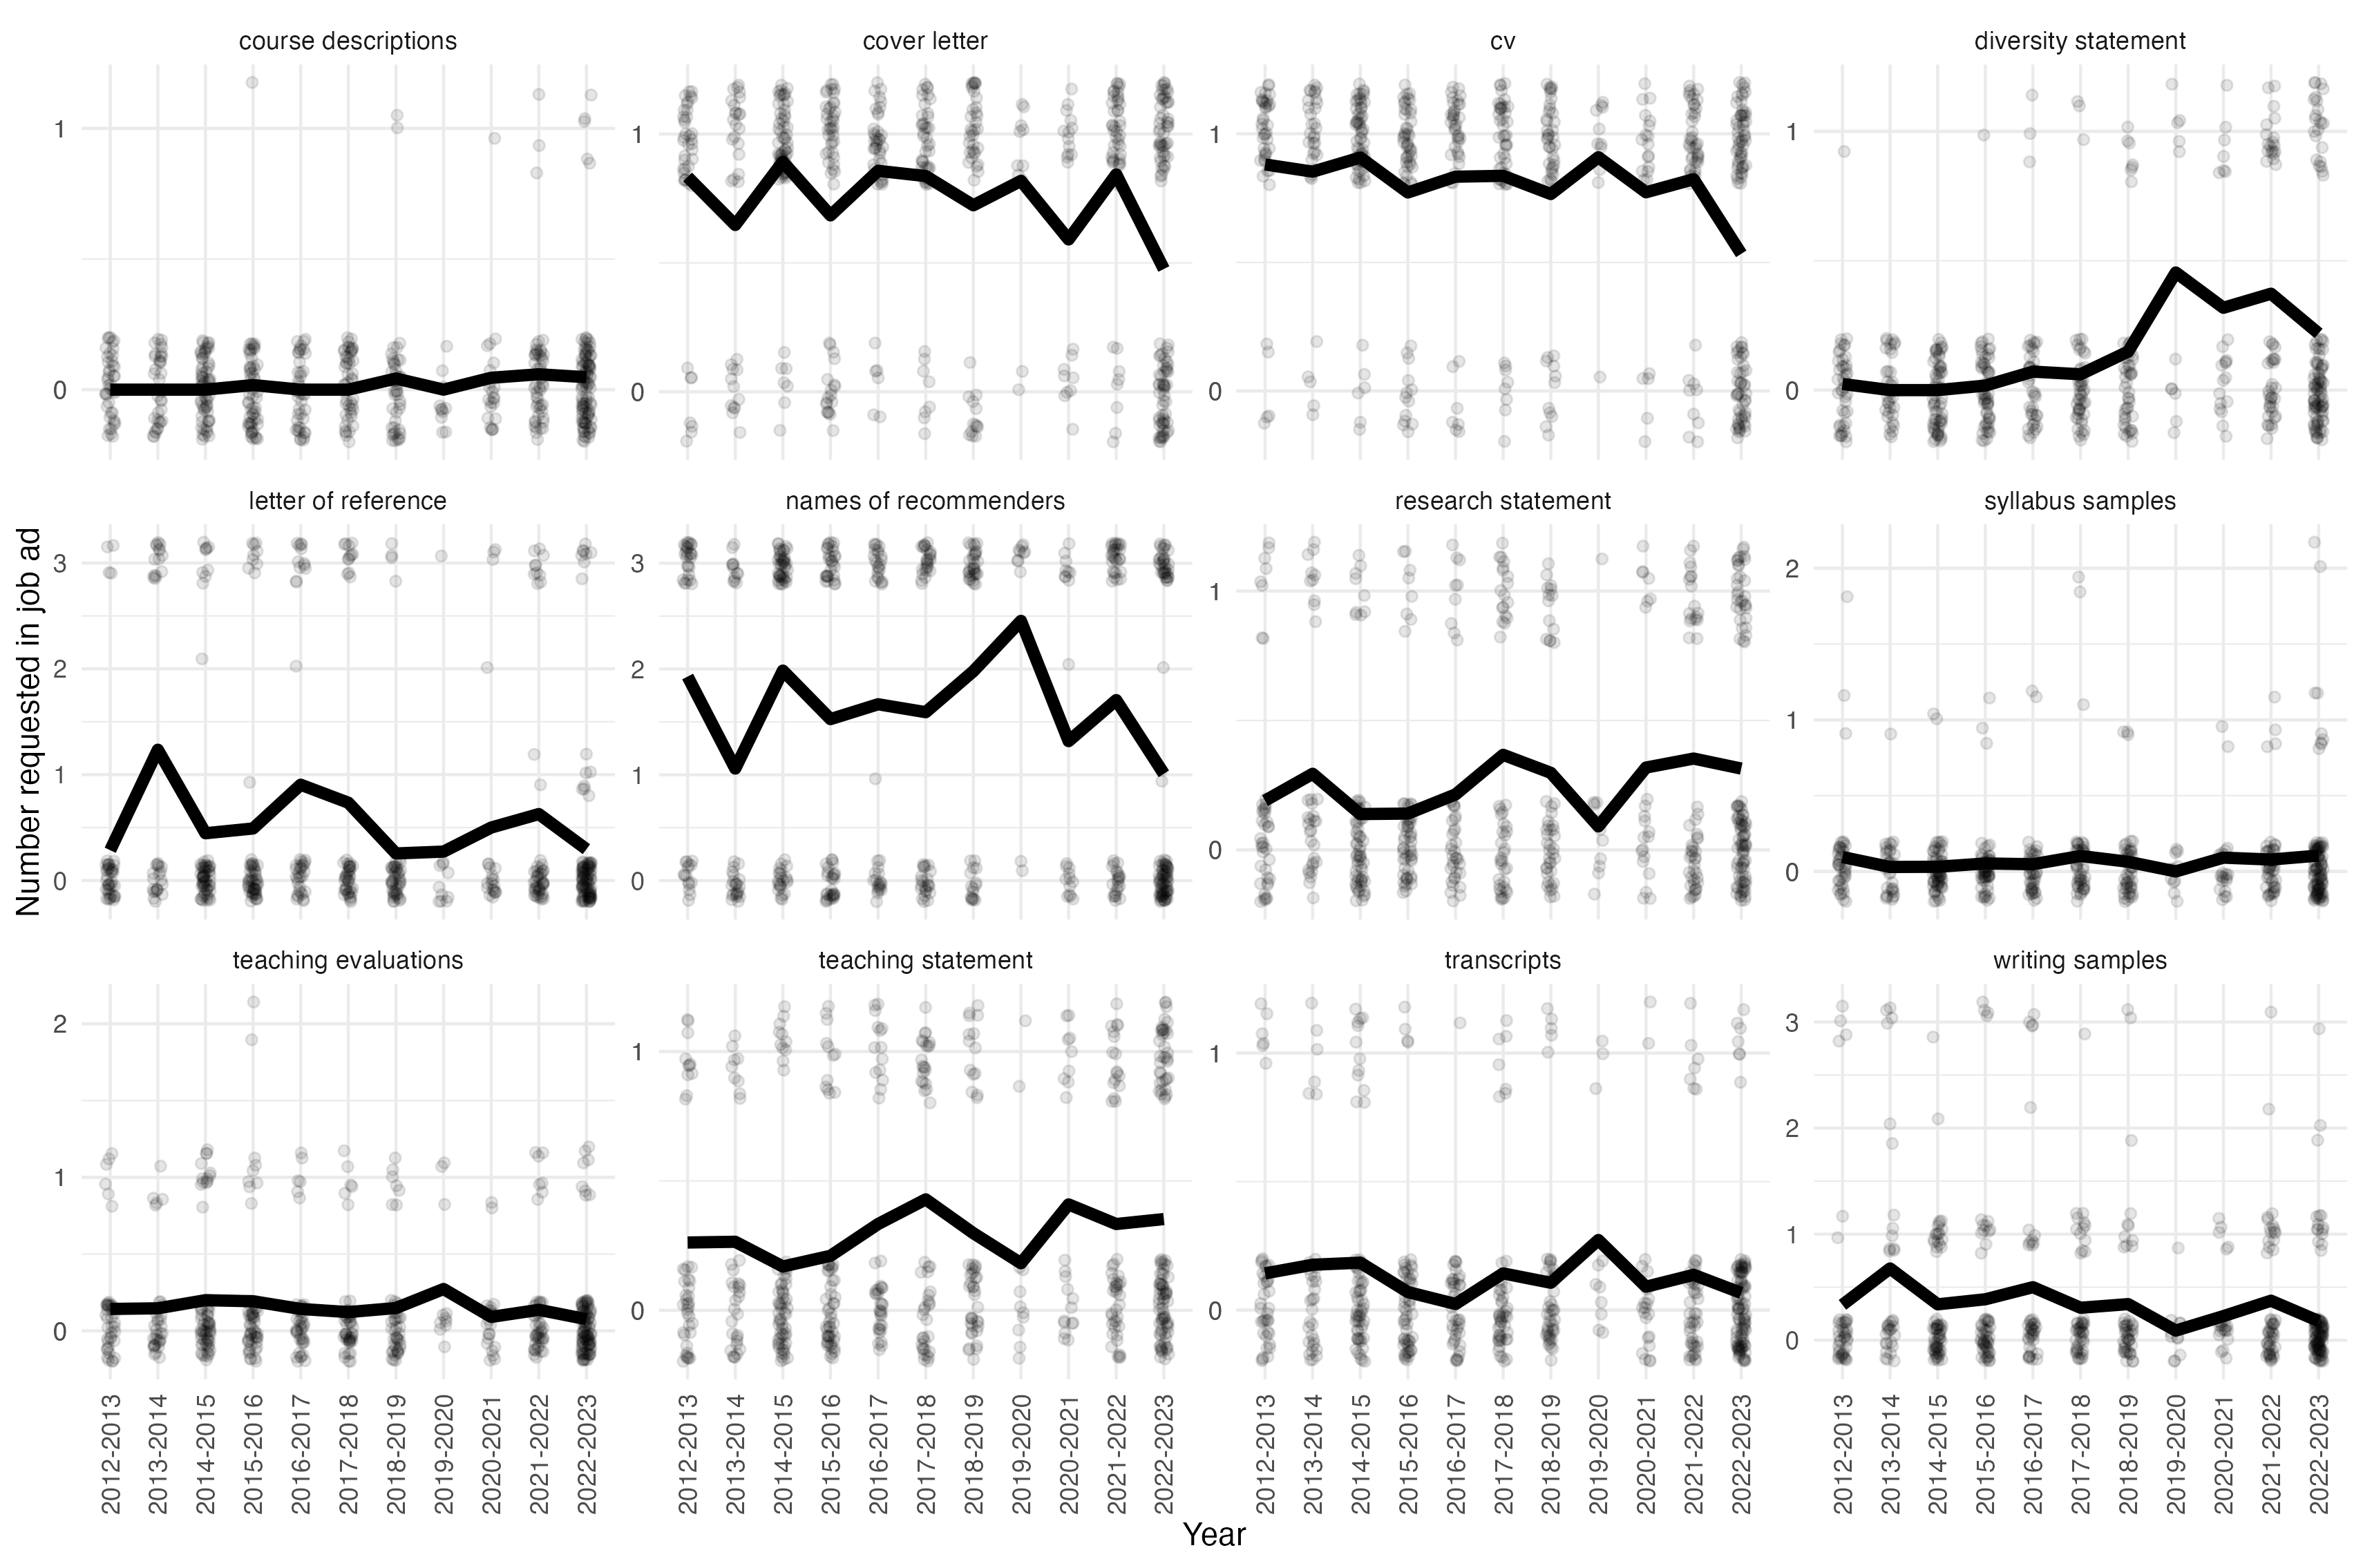
\includegraphics[width=10.8in,height=\textheight]{../figures/fig-requirements-per-year.png}

}

\caption{\label{fig-requirements-over-time}Changing requirements in job
ads over time. `Count' refers to the number of each item required.}

\end{figure}%

Over our ten year study period there have been substantial changes in
the instructions to applicants in terms of the type and number of
documents that are requested by the search committees
Figure~\ref{fig-requirements-over-time}. Requests for cover letter and
CV decline slightly in more recent years, perhaps reflecting their
status as a generic and expected component to submit without needing to
be specifically requested. The requirement for a diversity statement is
rare until 2019--2020, peaks around 2020--2021, then decreases towards
the present. Requests for names of recommenders (either zero or three
names, rarely only two names) reaches a maximum during 2019--2020, then
also decline for the remainder of the study period. The requirement for
a research statement and teaching statement increases after 2015--2016,
and becomes more frequent in job ads in more recent years. Requests for
course descriptions, syllabus samples, teaching evaluations, transcripts
and writing samples are consistently low over time (not shown here).

\section{Discussion}\label{discussion}

Our study of a decade of tenure-track job ads in archaeology in the U.S.
reveals diverse dynamics in the demand for specializations in topics,
methods and geographic focus, and in the instructions to applicants.
While these dynamics are familiar to scholars actively seeking faculty
positions, we believe this is the first time they have been quantified
at such a large scale within archaeology. Trends in job ads reflect
broader shifts in intellectual and practical priorities concerning
archaeology, undergraduate education, and the process of hiring
professors. The demand for archaeology faculty, indicated by the total
number of tenure-track jobs, may be affected by a variety of factors.

Overall, we found more tenure-track jobs advertised each year than
non-tenure-track, with the exception of 2013--2014. The wiki's emphasis
on tenure-track jobs runs counter to well-established patterns in the
academic job market, wherein short-term and contingent positions are
fast outpacing ``the last good job{[}s{]} in America'' (Aronowitz 2001).
Research across anthropological sub-fields has shown that the number of
tenure-track positions advertised within the discipline has also
declined. Analyzing the job ads posted in \emph{Anthropology News} in
1999--2000 versus 2019--2020, for example, Gershon and Rachok (2021)
found that the number of tenure-track positions decreased by 25\%
between their two time slices. Similarly, in his examination of jobs ads
posted on the Biological Anthropology Academic Jobs Wiki between
2010--2017, Passalacqua noted that approximately one quarter of the 474
ads posted were for adjunct or visiting staff (2018:773). Though
Passalacqua did not examine how the proportion of job types changed over
time, he did underscore ``a current diverging trend of decreasing
academic job advertisements and increasing doctoral degrees in
biological anthropology which could result in serious consequences for
the discipline'' (2018:773). Such observations have a surprising
longevity. Rogge raised the alarm nearly half a century ago, warning of
the ``maladaptive'' consequences of the exponential rate of disciplinary
growth and impending consequences for job seekers (Rogge 1976:839). The
dwindling number of permanent academic positions is not a trend unique
to anthropology---as of 2019, the AAUP documented a 36\% increase in
contingent positions over the preceding 15 years (AAUP 2022), and as of
2022, contingent positions make up more than half of faculty positions
in the United States (American Association of University Professors
2022b) .

This discrepancy in our data set---wherein advertisements for
tenure-track positions dominate the wiki despite their increasing rarity
in larger market---may be due to several factors. The first involves the
more limited circulation of advertising for short-term positions
relative to advertising for tenure-track jobs. Many of these short-term
positions are not advertised nationally, but are instead disseminated
through local email lists and are filled by people close to the hiring
department, such as recently graduated students. A second factor is bias
in our data---with most Wiki users likely seeking a tenure-track job,
non-tenure-track jobs may have been less frequently added to the
Academic Jobs Wiki because they were peripheral to the goal of most
users. This bias limits the reliability of our results on the ratio of
tenure-track to non-tenure-track positions. Tellingly, Passalacqua's
examination of a similar Wiki over a seven-year span showed a similar
dominance of permanent positions---291/474 (63\%) were for tenure-track
hires at various levels (2018: Table 2). This congruence between
subfields suggests that these patterns are a reflection of the Wiki,
rather than the market itself.

It is no secret that tenure-track jobs have traditionally been
considered the ``gold standard'' of career outcomes for PhD students in
the social sciences and humanities. As Kelsky outlines in \emph{The
Professor Is In}, her influential and best-selling guide for PhD
students pursuing faculty careers, ``\ldots most ranking graduate
programs still consider any PhD who doesn't land a tenure-track job a
failure or an aberration\ldots{} Graduate students absorb this value
system and judge themselves harshly'' (2015:11). These rubrics of
success have been common across the humanities and social sciences for
over half a century. Evaluating the demise of the National Endowment for
Humanities Funded ``Program to ready PhDs for Careers in Business''
(CIB), which aimed to facilitate humanities PhDs' transition to the
corporate world in the late 1970s, Franczak points to the dissonance
between participants' incentives and outcomes:

``The biggest lesson we can take from CIB is also the most obvious.
PhDs, especially in the humanities, want to be academics. The deep
reservoir of adjunct or contingent faculty that elite and non-elite
universities alike depend on for their courses is testament to this
fact---as is the excellent scholarship so many adjuncts produce without
department support. To pretend otherwise is disingenuous, and, as CIB
shows, possibly dangerous, too'' (Bessner and Brenes 2021:36).

The desire to pursue an academic career also characterizes more recent
PhD cohorts, including those within archaeology. Brami et al's survey
found that despite the long odds and professional precarity, 71\% of
their early career respondents wished to remain in academia (2023:242).
Overall, the obsessive valorization of permanent faculty positions in
the face of a precipitous decline in available jobs is indicative of the
potent combination of denial and delusion across academia. As Cefkin and
Schwegler argue ``This asymmetry between the `ideal' career path and the
experiences of most graduates highlights the deep and growing chasm
between the future that higher education institutions envision---and
strongly incentivize---and what is actually happening'' (Cefkin and
Schwegler 2024).

Returning to our results, the downward trend in tenure-track positions
during 2013--2019 may be related to declining undergraduate enrollment
in anthropology since 2013 (Cramb et al. 2022). The big dip during
2020--2021 is explained by the hiring freezes at many institutions
resulting from the COVID-19 pandemic, which caused extreme disruption
and uncertainty as universities focused on adapting to online
instruction and assessment in an effort to minimize the spread of the
virus (Woolston 2020). A survey of early career researchers in
archaeology captures the impact of this dip, with three-quarters of
respondents experiencing negative impacts on their careers due to the
pandemic (Brami et al. 2023).

The 2019--2021 period was also a major inflection point in the
popularity of specific topics and regions in job ads. Calls for
positions incorporating Indigenous and historical archaeology, and
archaeology of the Americas, became far more frequent at this time,
while Archaeological science, Complex societies, and the Mediterranean
and Near East showed declines in popularity. Similarly, the number of
job ads with a geographic focus on the Americas and Africa peaks during
2019--2021. These shifts in the topical and geographic foci of job ads
were likely influenced by broader cultural movements such as Black Lives
Matter, protests about racial injustice, and efforts to amplify
Indigenous voices (Dunivin et al. 2022; Flewellen et al. 2021; Franklin
et al. 2020; Laluk et al. 2022). COVID-19 also negatively impacted
Black, Indigenous American, and Hispanic communities with significantly
higher infection and morbidity rates, drawing attention to racial and
socio-economic inequality in the U.S. (Mackey et al. 2021; Tai et al.
2021). The Black Lives Matter movement, dating back to 2013, intersected
profoundly with the pandemic and the murder of George Floyd in
Minneapolis by a police officer in May 2020, three months after the
World Health Organization declared COVID-19 to be a pandemic. Mass
protests objecting to Floyd's murder generated widespread concern about
racial inequities and stimulated a broad interest in addressing systemic
racial injustice.

Our data suggest that archaeology faculty at U.S. universities
participated in this movement by adjusting their hiring plans to
prioritize recruiting archaeologists working on topics relevant to Black
and Indigenous communities. Many universities may have hoped to hire
Black and Indigenous archaeologists as part of their effort to tackle
systemic racism. Due to the Civil Rights Act of 1964 which prohibits
hiring based solely on race or ethnicity, however, it is illegal for
U.S. universities use race or ethnicity as a primary factor in hiring.
As a result, universities appear to have tailored the content of their
job ads to focus on topics where they expected Black and Indigenous
researchers to be most numerous, in an effort to ensure that these
researchers would be well-represented in the pool of applicants.

This striking change in topics and geographic foci of 2019--2021
occurred against a backdrop of several longer-term trends. Over the
course of the study period, we document a gradual decline in topics such
as Complex societies and Archaeological science, the geographic foci of
Mesoamerica and South America, and methods relating to Landscape
archaeology. These trends are harder to explain as we cannot link their
origins to a historical event such as the COVID-19 pandemic. We might
speculate that a growing preference for archaeological approaches that
privilege agency-driven, subjective, and relational perspectives is one
enduring legacy of debates in the 1980s and 90s about processualism
versus post-processualism (Fogelin 2019; Hodder 1999; Johnson 2019).
This theoretical trend might explain why archaeological science is
showing a decline, as demand for methods for analyzing artefact
materiality, ontology, and power displace physical laboratory methods
for technological, functional, and compositional analyses. Other factors
relevant to this decline may include the increasing difficulty of
obtaining research funding to support archaeological science research,
such as laboratory facilities and instrumentation. A decline in interest
in the archaeology of complex societies may reflect several themes that
intersect with broader social changes, such as growing interest in
Indigenous and non-state actors in the past and an increased concern
with climate change, environmental sustainability, and resilience,
shifting attention away from the study of monumental architecture, elite
societies, political hierarchies, and state systems.

Our data on the requirements for applicants support prior findings that
the complexity of applications---and concomitantly, the labor required
to apply for tenure-track jobs---has gradually increased over time. This
trend is especially pronounced for Assistant Professor positions, which
make more demands on applicants than Associate and Full Professor
positions. Consistent with results from other studies (Gershon and
Rachok 2021), our project documented a growing demand for research and
teaching statements. Demand for diversity statements shows a unique
trajectory, peaking in 2020--2021 and declining into the present. This
may relate to the intersecting concerns about race, identity and class
inequalities emerging during the COVID-19 pandemic, which seem to have
reached a peak in 2020--2021 and then declined over time, resulting in
jettisoning requests for diversity statements as the most urgent period
of the pandemic moves into the past. Another factor here may be the
debates surrounding the experiment with diversity statements in hiring
at some UC campuses during 2016--2022. Some universities that previously
required a diversity statement dropped that requirement after 2022
(Guiden 2024). In our data we observed a reversal of the diversity
statement requirement at 4 universities. Those schools posted job ads
prior 2022 that did require a diversity statement and also posted an ad
in 2022 that did not require one.

One bright spot for applicants is the decline in requests for names of
recommenders in the initial application in recent years. This may be a
response to recent criticisms of the burden on the applicant of
preparing numerous complex job applications (e.g. Dennis et al. 2022).
In recognition of this burden, not only on applicants but also on
colleagues writing letters of recommendation over and over to support
applicants, many hiring committees now follow the recommendations of
Dennis et al. (2022) in only requesting names and letters of
recommendation at later stages of the hiring process, if at all. Showing
sensitivity to this burden, in 2020 the American Anthropological
Association issued guidance to academic departments that letters of
recommendation should not be requested in the initial application, but
should only be required from short-listed candidates (American
Anthropological Association 2020; Youngling and Gershon 2020).

A key limitation of our research is that it does not include an analysis
of the academic profiles of those who were eventually hired based on
this sample of job ads. Our results reveal collective aspirations for
the future of the field, but only from those writing the job ads,
typically faculty who are securely employed as tenured professors
serving on hiring committees at U.S. colleges and universities. Our
results do not show how these aspirations worked out in the topical and
geographic foci of the people who were actually hired for these
positions. Future work should consider interviewing faculty hired during
our study period to match up scholars with the ads to which they
applied. If the successful applicants can be identified, then we could
analyze the fit between the details of the job ad and the applicant's
research. Such an analysis would allow us to assess how effective job
ads are for driving change in the discipline by setting the topics of
courses that will be taught in undergraduate and graduate curricula, and
research that will be supported by universities. We also recognize the
possibility that the Academic Jobs Wiki does not capture all available
positions and likely over-represents certain types of institutions.
Future work should evaluate these biases by comparing entries on the
Wiki to other sources of information about the academic job market, such
as the American Anthropological Association's AnthroGuide, or data
collected directly from universities.

\section{Conclusion}\label{conclusion}

The data introduced in this paper were initially collected and analyzed
in spring and summer 2024 and the manuscript was drafted in autumn 2024.
Between submitting the manuscript and receiving our initial round of
revisions in April 2025, the landscape of U.S. higher education has
shifted dramatically. The first hundred days of the new federal
administration focused on instilling a climate of ``economic precarity
and legal uncertainty'' across the sector through a cthuluesque strategy
that included withholding federal funding for colleges and universities,
decimating the Department of Education, revoking international student
visas, and attacking Diversity Equity, and Inclusion (DEI) initiatives
as ``unconstitutional'' (Knox and Alonso 2025). This deliberately
destabilizing ``flood the zone'' approach (Broadwater 2025) shows no
signs of abating. In April 2025, the U.S. president signed an executive
order to overhaul the higher education accreditation system (The White
House 2025), signifying the administration's continued commitment to
align higher education institutions to its ideological agenda.

Such challenges to the autonomy and self-governance in higher education
are particularly remarkable given that many architects of the current
administration hold degrees from the very institutions they are
attempting to dismantle, from Donald Trump (Wharton School of Business),
to J.D. Vance (Yale Law School), Chris Rufo (Georgetown), Stephen Miller
(Duke University), and Peter Hegseth (Harvard Kennedy School). Reviewing
the profiles of the board of trustees for the Heritage Foundation---the
conservative think tank which generated the Project 2025 report that has
been used as a blueprint for feeding U.S. higher education ``into a
woodchipper'' (Kunder 2025)---is also illustrative. Two thirds of the
trustees on the Heritage Foundation board have advanced degrees, while
one third have doctoral degrees from institutions such as Harvard,
Oxford, the University of Colorado, and the University of Texas. Lindsey
Burke, who authored the Project 2025 chapter on the Department of
Education, holds a PhD from George Mason University. Such career
trajectories are a testament to the elite chiasmus that decries the
merits and value of higher education while leveraging the credentials
granted by elite institutions for professional gain. As Ho notes of the
parallel systems of credentialing that undergird the ideology of
``smartness'' among Wall Street investment banks, playing the role of
``master of the universe'' requires both ``especially strong doses of
self-confidence and institutional legitimation'' (2009:41). Even
archaeology is susceptible to the power and pull of such prestige
hierarchies, which influence everything from hiring networks (Kawa et
al. 2019; Speakman, Hadden, Colvin, Cramb, Jones, Jones, Lulewicz, et
al. 2018) to publishing decisions (Beck et al. 2021) to research design
(Wobst and Keene 1983).

To echo Paul Farmer, ``all this is both interesting and horrible''
(2004:316). Contextualizing our job ad findings in this sociopolitical
tumult provokes a suite of new questions about academic futures. Many
archaeologists now have urgent concerns about what topics are likely to
be ``safe'' and lead to secure ongoing employment, considering the
current political and funding landscape. Will states with stronger
cultural and environmental regulations offer more stability in
employment, and if so, which states are likely to be the safest? These
are legitimate and crucial questions, but predicting the future goes
beyond the scope of our examination of the past decade of hiring
dynamics in academic archaeology. Extrapolating future trends is
inherently uncertain, especially in a mercurial political and economic
landscape that is experiencing tectonic shifts in bureaucracy,
organization, and funding on a near-weekly basis. Our study does,
however, point to at least four findings that have implications for the
next ten years of hiring, despite the turbulent political climate of
2024--2025.

First, the macroeconomic uncertainty induced by the increased tariffs
introduced in early 2025 is likely to have both short-term and long-term
implications that slow economic growth (Schneider 2025), with effects
that will seep into the higher education sector. The last two periods of
major economic upheaval in the U.S.---the Great Recession and the
COVID-19 pandemic---had pronounced and negative consequences for
colleges and universities. These consequences were visible even within
academic archaeology. Speakman, Hadden, Colvin, Cramb, Jones, Jones,
Lulewicz, et al. (2018), for example, show the precipitous decline in
the proportion of PhDs hired into tenure-track anthropology departments
after the last recession (see the steep decline in Figure 5 between 2007
and 2009), resulting in the ``increased use of {[}non-tenure track
faculty{]} by higher education institutions, and more anthropology
doctorates entering the workforce'' (2018:12). As our results
demonstrate, during academic year 2020--2021, only 12 tenure-track jobs
in archaeology were posted on the Wiki, a 70\% decrease relative to the
mean of 39 per year posted during our survey period
Table~\ref{tbl-show-basic-counts}. As Knox and Alonso (2025) highlight,
hiring freezes and program cuts are already coming into effect just four
months into the new administration. Given past patterns, it is likely
that increased tariffs will result in tenure-track positions in academic
archaeology becoming even more scarce, and faculty and students should
prepare for this. Whether this signals a death knell for the discipline
or an opportunity for re-envisioning and reconfiguring the field (Cefkin
and Schwegler 2024) is up for debate.

Second, our results show that hiring in academic archaeology is
responsive to larger cultural and political shifts. The increased
popularity of Indigenous and historical archaeology from 2019--2021
reflects the prominence and impact of movements such as Black Lives
Matter and a then-growing interest in conversations about race and
national history. The continual responsiveness to current events
revealed by our analysis of archaeology job ads demonstrates that our
narratives of the past are entangled in the social and political milieu
in which we work. This finding is consistent with previous
work---Trigger (1984) outlined how archaeological research programs are
shaped by national histories, while Soffer (1983), Blakey (1983),
Meltzer (1983), and Wilk (1985) have interrogated the entanglement of
identity, ideology, national history, politics, and archaeology across
space and time. Our study of job ads shows an active effort by
archaeologists to take control of interpreting the past, offering an
example of how disciplinary choices can shape archaeological research
programs. That said, in early 2025 many researchers had their work
disrupted by cancellations of funding from the U.S. National Science
Foundation if their projects contained certain keywords (Mervis 2025),
and others were told to cease activities if their projects contain
keywords such as ``cultural relevance,'' ``institutional,''
``historically,'' ``socioeconomic,'' and ``systemic'' (Johnson et al.
2025). This unprecedented keyword vetting suggests that future topical
shifts in archaeological research may be as much an individual response
to top-down funding pressures (cf. Wobst and Keene 1983) as a
disciplinary response to the current historical moment.

Third, the high chronological resolution of our analysis relative to
previous studies of disciplinary trends (e.g. Lyman 2010) shows that the
rise and fall of some of the foci we observed span relatively short
periods of time. This limits the predictive power of our results and has
implications for prospective graduate students and their mentors. A
topic that is growing in popularity as a student begins their PhD may
have peaked and be in decline before they graduate. Methods seem to have
a much lower frequency of change in popularity relative to topical and
geographic foci. One implication of this finding is that a graduate
student who has invested in developing technical expertise in a method
during their studies, in addition to a topic and region, might be less
vulnerable to the vagaries of the job market than a student without a
distinct area of technical expertise in generating data from material
records of past human behaviour.

Finally, our work also reveals the market forces that shaped the early
careers of the next generation of academic mentors. Assistant and
associate professors who experienced the academic market as job seekers
themselves between 2012--2023 probably anticipate that their students
will need publications, external grants, teaching experience, interview
preparation, extensive and tailored portfolios of job markets, and the
ability to spend many years on the market before obtaining a permanent
position, if they obtain one at all. This raises the question of whether
mentors' experiences on a market characterized by a recession and a
pandemic will be enough to guide their students through the volatility
of the next decade, and how they should update their programs to prepare
their graduates for success.

\section{Acknowledgements}\label{acknowledgements}

Thanks to the anonymous contributors to the Academic Jobs Wiki, without
whose efforts to collect and organise hundreds of job ads, this paper
would not exist. To those of you who contributed to the wiki but did not
obtain a tenure-track job, and/or decided to pivot to another industry,
we hope this paper shows your time on the wiki was not wasted. Your
efforts have helped contribute to more accurate expectation-setting for
future generations of archaeologists.

\section{Data Availability Statement}\label{data-availability-statement}

The data that support the findings of this study are openly available in
Zenodo at https://doi.org/10.5281/zenodo.14798941

\section{Funding Statement}\label{funding-statement}

This research received no specific grant funding from any funding
agency, commercial or not-for-profit sectors.

\section{Competing Interests
Statement}\label{competing-interests-statement}

Competing interests: The authors declare none

\section{Supplementary materials}\label{supplementary-materials}

Our supplementary materials are available at
https://doi.org/10.5281/zenodo.14798941

\newpage

\section{References cited}\label{references-cited}

\phantomsection\label{refs}
\begin{CSLReferences}{0}{1}
\bibitem[\citeproctext]{ref-jobboar2020}
\CSLBlock{American Anthropological Association}
\CSLLeftMargin{ 2020}%
\CSLRightInline{Job board policies.
\url{https://employers.americananthro.org/static-page/10285/job-board-policies/},
accessed January 26, 2025.}

\bibitem[\citeproctext]{ref-colby2022annual}
\CSLBlock{American Association of University Professors}
\CSLLeftMargin{ 2022b}%
\CSLRightInline{The annual report on the economic status of the
profession, 2021--22. American Association of University Professors.
\url{https://www.aaup.org/report/annual-report-economic-status-profession-2021-22},
accessed January 26, 2025.}

\bibitem[\citeproctext]{ref-the20222022}
\CSLLeftMargin{ 2022a }%
\CSLRightInline{The 2022 AAUP survey of tenure practices.
\url{https://www.aaup.org/report/2022-aaup-survey-tenure-practices},
accessed January 26, 2025.}

\bibitem[\citeproctext]{ref-aronowitz2001}
\CSLBlock{Aronowitz, Stanley}
\CSLLeftMargin{ 2001}%
\CSLRightInline{\emph{The last good job in america: Work and education
in the new global technoculture}. Critical perspectives series. Rowman
\& Littlefield : Distributed by National Book Network, Lanham, Md.}

\bibitem[\citeproctext]{ref-barnett2010}
\CSLBlock{Barnett, George A., James A. Danowski, Thomas Hugh Feeley, and
Jordan Stalker}
\CSLLeftMargin{ 2010}%
\CSLRightInline{Measuring quality in communication doctoral education
using network analysis of faculty-hiring patterns. \emph{Journal of
Communication} 60(2):388--411.
DOI:\href{https://doi.org/10.1111/j.1460-2466.2010.01487.x}{10.1111/j.1460-2466.2010.01487.x}.}

\bibitem[\citeproctext]{ref-barrett2008mediawiki}
\CSLBlock{Barrett, Daniel J}
\CSLLeftMargin{ 2008}%
\CSLRightInline{\emph{MediaWiki}. O'Reilly Media, Inc.}

\bibitem[\citeproctext]{ref-beck}
\CSLBlock{Beck, Jess}
\CSLLeftMargin{ 2025}%
\CSLRightInline{Stubborn architecture: The jobs crisis in academic
anthropology. In. SAR Press, in press, Santa Fe.}

\bibitem[\citeproctext]{ref-beck2021}
\CSLBlock{Beck, Jess, Erik Gjesfjeld, and Stephen Chrisomalis}
\CSLLeftMargin{ 2021}%
\CSLRightInline{Prestige or Perish: Publishing Decisions in Academic
Archaeology. \emph{American Antiquity} 86(4):669--695.
DOI:\href{https://doi.org/10.1017/aaq.2021.64}{10.1017/aaq.2021.64}.}

\bibitem[\citeproctext]{ref-bessner2021}
\CSLBlock{Bessner, Daniel, and Michael Brenes}
\CSLLeftMargin{ 2021}%
\CSLRightInline{The academic jobs crisis: A forum. \emph{Passport: The
Society for Historians of American Foreign Relations Review}
52(1):3053.}

\bibitem[\citeproctext]{ref-blakey1983}
\CSLBlock{Blakey, Michael}
\CSLLeftMargin{ 1983}%
\CSLRightInline{Socio-political bias and ideological production in
historical archaeology. In, edited by Joan M. Gero, David M. Lacy, and
Michael L. Blakey, pp. 5--16. Research reports, department of
anthropology. University of Massachusetts, Amherst.}

\bibitem[\citeproctext]{ref-bramiPrecariousFutureReflections2023}
\CSLBlock{Brami, Maxime, Stephanie Emra, Antoine Muller, Bianca
Preda-Bălănică, Benjamin Irvine, Bogdana Milić, Aldo Malagó, Katie
Meheux, and Manuel Fernández-Götz}
\CSLLeftMargin{ 2023}%
\CSLRightInline{A precarious future: Reflections from a survey of early
career researchers in archaeology. \emph{European Journal of
Archaeology} 26(2):226--250.
DOI:\href{https://doi.org/10.1017/eaa.2022.41}{10.1017/eaa.2022.41}.}

\bibitem[\citeproctext]{ref-broadwater2025}
\CSLBlock{Broadwater, Luke}
\CSLLeftMargin{ 2025}%
\CSLRightInline{\href{https://www.nytimes.com/2025/01/28/us/politics/trump-policy-blitz.html}{Trump{'}s
{`}flood the zone{'} strategy leaves opponents gasping in outrage}.
\emph{The New York Times}.}

\bibitem[\citeproctext]{ref-castillo}
\CSLBlock{Castillo, Enrique del, Adam Meyers, and Peng Chen}
\CSLLeftMargin{ 2018}%
\CSLRightInline{A Social Network Analysis of the Operations
Research/Industrial Engineering Faculty Hiring Network. \emph{preprint
on arXiv.org}.
DOI:\href{https://doi.org/10.48550/arXiv.1803.00125}{10.48550/arXiv.1803.00125}.}

\bibitem[\citeproctext]{ref-cefkin}
\CSLBlock{Cefkin, Melissa, and Tara Schwegler}
\CSLLeftMargin{ 2024}%
\CSLRightInline{\href{https://www.insidehighered.com/opinion/career-advice/2024/05/09/graduate-work-must-focus-both-academic-and-applied-opinion}{A
nonapocalyptic vision of graduate education{'}s future}. \emph{Inside
Higher Ed}.}

\bibitem[\citeproctext]{ref-clauset2015}
\CSLBlock{Clauset, Aaron, Samuel Arbesman, and Daniel B. Larremore}
\CSLLeftMargin{ 2015}%
\CSLRightInline{Systematic inequality and hierarchy in faculty hiring
networks. \emph{Science Advances} 1(1):e1400005.
DOI:\href{https://doi.org/10.1126/sciadv.1400005}{10.1126/sciadv.1400005}.}

\bibitem[\citeproctext]{ref-crambChangingProfileTenureTrack2022a}
\CSLBlock{Cramb, Justin, Brandon T. Ritchison, Carla S. Hadden, Qian
Zhang, Edgar Alarcón-Tinajero, Xianyan Chen, K. C. Jones, Travis Jones,
Katharine Napora, Matthew Veres, and Victor D. Thompson}
\CSLLeftMargin{ 2022}%
\CSLRightInline{The changing profile of tenure-track faculty in
archaeology. \emph{Advances in Archaeological Practice} 10(4):371--381.
DOI:\href{https://doi.org/10.1017/aap.2022.8}{10.1017/aap.2022.8},
accessed October 16, 2024.}

\bibitem[\citeproctext]{ref-culver}
\CSLBlock{Culver, KC, and Adrianna Kezar}
\CSLLeftMargin{ 2022}%
\CSLRightInline{\href{https://doi.org/10.17226/26405}{The impacts of
2020 on advancement of non-tenure-track and adjunct faculty}. In
\emph{Promotion, tenure, and advancement through the lens of 2020:
Proceedings of a workshop---in brief}, edited by Maria Lund Dahlberg,
pp. 16--19. National Academies of Sciences, Engineering,; Medicine.}

\bibitem[\citeproctext]{ref-dennisWorstAnthroJob2022}
\CSLBlock{Dennis, Dannah, Dada Docot, Danielle Gendron, and Ilana
Gershon}
\CSLLeftMargin{ 2022}%
\CSLRightInline{The worst of anthro job ads for 2021. \emph{American
Anthropologist} 124(4):900--905.
DOI:\href{https://doi.org/10.1111/aman.13781}{10.1111/aman.13781},
accessed October 22, 2024.}

\bibitem[\citeproctext]{ref-dunivinBlackLivesMatter2022}
\CSLBlock{Dunivin, Zackary Okun, Harry Yaojun Yan, Jelani Ince, and
Fabio Rojas}
\CSLLeftMargin{ 2022}%
\CSLRightInline{Black lives matter protests shift public discourse.
\emph{Proceedings of the National Academy of Sciences}
119(10):e2117320119.
DOI:\href{https://doi.org/10.1073/pnas.2117320119}{10.1073/pnas.2117320119}.}

\bibitem[\citeproctext]{ref-earle2014}
\CSLBlock{Earle, Beverley, and Marianne DelPo Kulow}
\CSLLeftMargin{ 2014}%
\CSLRightInline{The {"}Deeply Toxic{"} Damage Caused by the Abolition of
Mandatory Retirement and Its Collision with Tenure in Higher Education:
A Proposal for Statutory Repair. \emph{Southern California
Interdisciplinary Law Journal}:369--418.}

\bibitem[\citeproctext]{ref-farmer2004}
\CSLBlock{Farmer, Paul}
\CSLLeftMargin{ 2004}%
\CSLRightInline{An Anthropology of Structural Violence. \emph{Current
Anthropology} 45(3):305--325.
DOI:\href{https://doi.org/10.1086/382250}{10.1086/382250}.}

\bibitem[\citeproctext]{ref-feeley2021}
\CSLBlock{Feeley, Thomas Hugh, and Frank Tutzauer}
\CSLLeftMargin{ 2021}%
\CSLRightInline{The faculty hiring network for PhD-granting
communication programs. \emph{Scientometrics} 126(5):3983--4003.
DOI:\href{https://doi.org/10.1007/s11192-021-03917-y}{10.1007/s11192-021-03917-y}.}

\bibitem[\citeproctext]{ref-flewellenFutureArchaeologyAntiracist2021}
\CSLBlock{Flewellen, Ayana Omilade, Justin P. Dunnavant, Alicia Odewale,
Alexandra Jones, Tsione Wolde-Michael, Zoë Crossland, and Maria
Franklin}
\CSLLeftMargin{ 2021}%
\CSLRightInline{{``}The Future of Archaeology Is Antiracist{''}:
Archaeology in the Time of Black Lives Matter. \emph{American Antiquity}
86(2):224--243.
DOI:\href{https://doi.org/10.1017/aaq.2021.18}{10.1017/aaq.2021.18}.}

\bibitem[\citeproctext]{ref-Fogelin2019}
\CSLBlock{Fogelin, Lars}
\CSLLeftMargin{ 2019}%
\CSLRightInline{An unauthorized companion to american archaeological
theory. Self-published. \url{https://arizona.academia.edu/LarsFogelin},
accessed January 26, 2025.}

\bibitem[\citeproctext]{ref-franklinFutureNowArchaeology2020}
\CSLBlock{Franklin, Maria, Justin P. Dunnavant, Ayana Omilade Flewellen,
and Alicia Odewale}
\CSLLeftMargin{ 2020}%
\CSLRightInline{The Future is Now: Archaeology and the Eradication of
Anti-Blackness. \emph{International Journal of Historical Archaeology}
24(4):753--766.
DOI:\href{https://doi.org/10.1007/s10761-020-00577-1}{10.1007/s10761-020-00577-1}.}

\bibitem[\citeproctext]{ref-HelloTristesTropes2021}
\CSLBlock{Gershon, Ilana, and Dafna Rachok}
\CSLLeftMargin{ 2021}%
\CSLRightInline{Hello to {Tristes Tropes}. Anthropology News.
\url{https://www.anthropology-news.org/articles/hello-to-tristes-tropes/},
accessed August 2, 2022.}

\bibitem[\citeproctext]{ref-Ghaffarzadegan_2015}
\CSLBlock{Ghaffarzadegan, Navid, Joshua Hawley, Richard Larson, and Yi
Xue}
\CSLLeftMargin{ 2015}%
\CSLRightInline{A note on PhD population growth in biomedical sciences.
\emph{Systems Research and Behavioral Science} 32(3):402--405.
DOI:\href{https://doi.org/10.1002/sres.2324}{10.1002/sres.2324}.}

\bibitem[\citeproctext]{ref-graeber2018}
\CSLBlock{Graeber, David}
\CSLLeftMargin{ 2018}%
\CSLRightInline{\emph{Bullshit jobs}. Simon \& Schuster, New York.}

\bibitem[\citeproctext]{ref-griffin2000native}
\CSLBlock{Griffin-Pierce, Trudy}
\CSLLeftMargin{ 2000}%
\CSLRightInline{\emph{Native peoples of the southwest}. UNM Press.}

\bibitem[\citeproctext]{ref-guidenAreDiversityStatements}
\CSLBlock{Guiden, Mary}
\CSLLeftMargin{ 2024}%
\CSLRightInline{Are diversity statements a thing of the past? Harvard is
the latest to drop this requirement for job applicants.
\url{https://www.higheredjobs.com/Articles/articleDisplay.cfm?ID=3948},
accessed November 1, 2024.}

\bibitem[\citeproctext]{ref-gusterson2017}
\CSLBlock{Gusterson, Hugh}
\CSLLeftMargin{ 2017}%
\CSLRightInline{Homework: Toward a critical ethnography of the
university: AES presidential address, 2017. \emph{American Ethnologist}
44(3):435--450.
DOI:\href{https://doi.org/10.1111/amet.12520}{10.1111/amet.12520}.}

\bibitem[\citeproctext]{ref-ho2009}
\CSLBlock{Ho, Karen Zouwen}
\CSLLeftMargin{ 2009}%
\CSLRightInline{\emph{Liquidated : An ethnography of wall street}. Duke
University Press, Durham.}

\bibitem[\citeproctext]{ref-hodderArchaeologicalProcessIntroduction1999}
\CSLBlock{Hodder, Ian}
\CSLLeftMargin{ 1999}%
\CSLRightInline{\emph{The archaeological process: An introduction}.
Blackwell, Oxford.}

\bibitem[\citeproctext]{ref-johnson2025}
\CSLBlock{Johnson, Carolyn Y., Scott Dance, and Joel Achenbach}
\CSLLeftMargin{ 2025}%
\CSLRightInline{\href{https://www.washingtonpost.com/science/2025/02/04/national-science-foundation-trump-executive-orders-words/}{Here
are the words putting science in the crosshairs of trump{'}s orders}.
\emph{The Washington Post}.}

\bibitem[\citeproctext]{ref-johnson2019archaeological}
\CSLBlock{Johnson, Matthew}
\CSLLeftMargin{ 2019}%
\CSLRightInline{\emph{Archaeological theory: An introduction}. John
Wiley \& Sons.}

\bibitem[\citeproctext]{ref-kaskie2016}
\CSLBlock{Kaskie, Brian}
\CSLLeftMargin{ 2016}%
\CSLRightInline{The Academy Is Aging in Place: Assessing Alternatives
for Modifying Institutions of Higher Education. \emph{The
Gerontologist}:gnw001.
DOI:\href{https://doi.org/10.1093/geront/gnw001}{10.1093/geront/gnw001}.}

\bibitem[\citeproctext]{ref-kawaSocialNetworkUS2019}
\CSLBlock{Kawa, Nicholas C., José A. Clavijo Michelangeli, Jessica L.
Clark, Daniel Ginsberg, and Christopher McCarty}
\CSLLeftMargin{ 2019}%
\CSLRightInline{The {Social Network} of {US Academic Anthropology} and
{Its Inequalities}. \emph{American Anthropologist} 121(1):14--29.
DOI:\href{https://doi.org/10.1111/aman.13158}{10.1111/aman.13158},
accessed October 31, 2024.}

\bibitem[\citeproctext]{ref-kelsky2015}
\CSLBlock{Kelsky, Karen}
\CSLLeftMargin{ 2015}%
\CSLRightInline{\emph{The professor is in: The essential guide to
turning your ph.d. Into a job}. Three Rivers Press, New York.}

\bibitem[\citeproctext]{ref-knox2025}
\CSLBlock{Knox, Liam, and Johanna Alonso}
\CSLLeftMargin{ 2025}%
\CSLRightInline{\href{https://www.insidehighered.com/news/government/politics-elections/2025/04/30/how-trumps-first-100-days-transformed-higher-ed}{Trump{'}s
100-day war on higher ed}. \emph{Inside Highe Ed}.}

\bibitem[\citeproctext]{ref-kuckartz2014qualitative}
\CSLBlock{Kuckartz, Udo}
\CSLLeftMargin{ 2014}%
\CSLRightInline{\emph{Qualitative text analysis: A guide to methods,
practice and using software}. Sage.}

\bibitem[\citeproctext]{ref-lalukArchaeologySocialJustice2022}
\CSLBlock{Laluk, Nicholas C., Lindsay M. Montgomery, Rebecca Tsosie,
Christine McCleave, Rose Miron, Stephanie Russo Carroll, Joseph Aguilar,
Ashleigh Big Wolf Thompson, Peter Nelson, Jun Sunseri, Isabel Trujillo,
GeorgeAnn M. DeAntoni, Greg Castro, and Tsim D. Schneider}
\CSLLeftMargin{ 2022}%
\CSLRightInline{Archaeology and Social Justice in Native America.
\emph{American Antiquity} 87(4):659--682.
DOI:\href{https://doi.org/10.1017/aaq.2022.59}{10.1017/aaq.2022.59}.}

\bibitem[\citeproctext]{ref-larson2014}
\CSLBlock{Larson, Richard C., Navid Ghaffarzadegan, and Yi Xue}
\CSLLeftMargin{ 2014}%
\CSLRightInline{Too Many PhD Graduates or Too Few Academic Job Openings:
The Basic Reproductive Number R0 in Academia. \emph{Systems Research and
Behavioral Science} 31(6):745--750.
DOI:\href{https://doi.org/10.1002/sres.2210}{10.1002/sres.2210}.}

\bibitem[\citeproctext]{ref-lightfoot2021preparing}
\CSLBlock{Lightfoot, Elizabeth, Cynthia Franklin, and Raiza Beltran}
\CSLLeftMargin{ 2021}%
\CSLRightInline{Preparing for the academic job market: A guide for
social work doctoral students and their mentors. \emph{Journal of Social
Work Education} 57(1):153--164.}

\bibitem[\citeproctext]{ref-lyman2010american}
\CSLBlock{Lyman, R Lee}
\CSLLeftMargin{ 2010}%
\CSLRightInline{American archaeology textbooks as reflections of the
history of the discipline. \emph{North American Archaeologist}
31(1):1--25.}

\bibitem[\citeproctext]{ref-mackeyRacialEthnicDisparities2021}
\CSLBlock{Mackey, Katherine, Chelsea K. Ayers, Karli K. Kondo, Somnath
Saha, Shailesh M. Advani, Sarah Young, Hunter Spencer, Max Rusek,
Johanna Anderson, Stephanie Veazie, Mia Smith, and Devan Kansagara}
\CSLLeftMargin{ 2021}%
\CSLRightInline{Racial and ethnic disparities in
COVID-19{\textendash}related infections, hospitalizations, and deaths.
\emph{Annals of Internal Medicine} 174(3):362--373.
DOI:\href{https://doi.org/10.7326/M20-6306}{10.7326/M20-6306}.}

\bibitem[\citeproctext]{ref-mackieMarketShareAccounting2023}
\CSLBlock{Mackie, Madeline E., and Heather Rockwell}
\CSLLeftMargin{ 2023}%
\CSLRightInline{Beyond market share: Accounting for doctoral program
size in recent rates of anthropology faculty job placement. \emph{PLOS
ONE} 18(5):e0285330.
DOI:\href{https://doi.org/10.1371/journal.pone.0285330}{10.1371/journal.pone.0285330}.}

\bibitem[\citeproctext]{ref-main2019}
\CSLBlock{Main, Joyce B., Sarah Prenovitz, and Ronald G. Ehrenberg}
\CSLLeftMargin{ 2019}%
\CSLRightInline{In Pursuit of a Tenure-Track Faculty Position: Career
Progression and Satisfaction of Humanities and Social Sciences
Doctorates. \emph{The Review of Higher Education} 42(4):1309--1336.
DOI:\href{https://doi.org/10.1353/rhe.2019.0067}{10.1353/rhe.2019.0067}.}

\bibitem[\citeproctext]{ref-Marwick2017}
\CSLBlock{Marwick, Ben}
\CSLLeftMargin{ 2017}%
\CSLRightInline{Computational reproducibility in archaeological
research: Basic principles and a case study of their implementation.
\emph{Journal of Archaeological Method and Theory} 24(2):424--450.
DOI:\href{https://doi.org/10.1007/s10816-015-9272-9}{10.1007/s10816-015-9272-9}.}

\bibitem[\citeproctext]{ref-meltzer1983}
\CSLBlock{Meltzer, David}
\CSLLeftMargin{ 1983}%
\CSLRightInline{Prehistory, power and politics in the bureau of american
ethnology, 1879{\textendash}1906. In, edited by Joan M. Gero, David M.
Lacy, and Michael L. Blakey, pp. 6777. Research reports, department of
anthropology. University of Massachusetts, Amherst.}

\bibitem[\citeproctext]{ref-Mervis}
\CSLBlock{Mervis, Jeffrey}
\CSLLeftMargin{ 2025}%
\CSLRightInline{NSF's grant cuts fall heaviest on scientists from
underrepresented groups.
\url{https://www.science.org/content/article/nsf-s-grant-cuts-fall-heaviest-scientists-underrepresented-groups}.}

\bibitem[\citeproctext]{ref-mirowski2011}
\CSLBlock{Mirowski, Philip}
\CSLLeftMargin{ 2011}%
\CSLRightInline{\emph{Science-mart: Privatizing american science}.
Harvard University Press, Cambridge, Mass.}

\bibitem[\citeproctext]{ref-morganReadyNotArchaeological2023}
\CSLBlock{Morgan, Rachel}
\CSLLeftMargin{ 2023}%
\CSLRightInline{Ready or Not: An Archaeological Knowledge, Skills, and
Abilities Needs Assessment. \emph{Advances in Archaeological Practice}
11(4):371--387.
DOI:\href{https://doi.org/10.1017/aap.2023.21}{10.1017/aap.2023.21}.}

\bibitem[\citeproctext]{ref-musial2018five}
\CSLBlock{Musial, Jennifer, and Christina Holmes}
\CSLLeftMargin{ 2018}%
\CSLRightInline{Five-year study on hiring trends in gender, women's, and
feminist studies. \emph{Feminist Studies} 44(2):253--272.}

\bibitem[\citeproctext]{ref-IPEDSNCES}
\CSLBlock{National Center for Education Statistics}
\CSLLeftMargin{ 2025}%
\CSLRightInline{Integrated postsecondary education data system (IPEDS).
U.S. Department of Education. \url{https://nces.ed.gov/ipeds/}, accessed
January 25, 2025.}

\bibitem[\citeproctext]{ref-nevin2019}
\CSLBlock{Nevin, Andrew D.}
\CSLLeftMargin{ 2019}%
\CSLRightInline{Academic Hiring Networks and Institutional Prestige: A
Case Study of Canadian Sociology. \emph{Canadian Review of
Sociology/Revue canadienne de sociologie} 56(3):389--420.
DOI:\href{https://doi.org/10.1111/cars.12252}{10.1111/cars.12252}.}

\bibitem[\citeproctext]{ref-Passalacqua_2018}
\CSLBlock{Passalacqua, Nicholas V.}
\CSLLeftMargin{ 2018}%
\CSLRightInline{Are careers in biological anthropology sustainable?
\emph{American Journal of Physical Anthropology} 166(3):772--776.
DOI:\href{https://doi.org/10.1002/ajpa.23457}{10.1002/ajpa.23457}.}

\bibitem[\citeproctext]{ref-platzerAcademicPrecarityAmerican2018}
\CSLBlock{Platzer, David, and Anne Allison}
\CSLLeftMargin{ 2018}%
\CSLRightInline{Academic {Precarity} in {American Anthropology}. Society
for Cultural Anthropology.
\url{https://culanth.org/fieldsights/academic-precarity-in-american-anthropology},
accessed October 31, 2024.}

\bibitem[\citeproctext]{ref-rlanguage}
\CSLBlock{R Core Team}
\CSLLeftMargin{ 2024}%
\CSLRightInline{\emph{\href{https://www.R-project.org/}{R: A language
and environment for statistical computing}}. R Foundation for
Statistical Computing, Vienna, Austria.}

\bibitem[\citeproctext]{ref-rabinow1992}
\CSLBlock{Rabinow, Paul}
\CSLLeftMargin{ 1992}%
\CSLRightInline{For hire: Resolutely late modern. In, pp. 5971. School
of American Research Press, Santa Fe.}

\bibitem[\citeproctext]{ref-ribeiro2023}
\CSLBlock{Ribeiro, Artur, and Christos Giamakis}
\CSLLeftMargin{ 2023}%
\CSLRightInline{On Class and Elitism in Archaeology. \emph{Open
Archaeology} 9(1):20220309.
DOI:\href{https://doi.org/10.1515/opar-2022-0309}{10.1515/opar-2022-0309}.}

\bibitem[\citeproctext]{ref-rogge1976}
\CSLBlock{Rogge, A. E.}
\CSLLeftMargin{ 1976}%
\CSLRightInline{A Look at Academic Anthropology: Through a Graph Darkly.
\emph{American Anthropologist} 78(4):829--843.
DOI:\href{https://doi.org/10.1525/aa.1976.78.4.02a00070}{10.1525/aa.1976.78.4.02a00070}.}

\bibitem[\citeproctext]{ref-ryan2003techniques}
\CSLBlock{Ryan, Gery W, and H Russell Bernard}
\CSLLeftMargin{ 2003}%
\CSLRightInline{Techniques to identify themes. \emph{Field methods}
15(1):85--109.}

\bibitem[\citeproctext]{ref-schneider2025}
\CSLBlock{Schneider, Howard}
\CSLLeftMargin{ 2025}%
\CSLRightInline{\href{https://www.reuters.com/markets/us/feds-powell-weigh-amid-tariff-fray-market-drop-2025-04-04/}{Fed{'}s
powell says larger-than-expected tariffs likely to boost inflation, slow
growth}. \emph{Reuters}.}

\bibitem[\citeproctext]{ref-shulman2001carnegie}
\CSLBlock{Shulman, Lee S}
\CSLLeftMargin{ 2001}%
\CSLRightInline{\emph{The {C}arnegie classification of institutions of
higher education}. The Carnegie Foundation for the Advancement of
Teaching, California.}

\bibitem[\citeproctext]{ref-soffer1983}
\CSLBlock{Soffer, Olga}
\CSLLeftMargin{ 1983}%
\CSLRightInline{Politics of the paleolithic in the USSR: A case of
paradigms lost. In, edited by Joan M. Gero, David M. Lacy, and Michael
L. Blakey, pp. 91105. Research reports, department of anthropology.
University of Massachusetts, Amherst.}

\bibitem[\citeproctext]{ref-soucek2021diversity}
\CSLBlock{Soucek, Brian}
\CSLLeftMargin{ 2022}%
\CSLRightInline{\href{https://lawreview.law.ucdavis.edu/archives/55/4/diversity-statements.html}{Diversity
statements}. \emph{University of California Davis Law Review}
55:1989--2050.}

\bibitem[\citeproctext]{ref-speakman2018choosing}
\CSLBlock{Speakman, Robert J., Carla S. Hadden, Matthew H. Colvin,
Justin Cramb, K. C. Jones, Travis W. Jones, Corbin L Kling, Isabelle
Lulewicz, Katharine G. Napora, Katherine L. Reinberger, and others}
\CSLLeftMargin{ 2018}%
\CSLRightInline{Choosing a path to the ancient world in a modern market:
The reality of faculty jobs in archaeology. \emph{American Antiquity}
83(1):1--12.}

\bibitem[\citeproctext]{ref-speakman2018}
\CSLBlock{Speakman, Robert J., Carla S. Hadden, Matthew H. Colvin,
Justin Cramb, K. C. Jones, Travis W. Jones, Isabelle Lulewicz, Katharine
G. Napora, Katherine L. Reinberger, Brandon T. Ritchison, Alexandra R.
Edwards, and Victor D. Thompson}
\CSLLeftMargin{ 2018}%
\CSLRightInline{Market share and recent hiring trends in anthropology
faculty positions. Edited by John P. Hart. \emph{PLOS ONE}
13(9):e0202528.
DOI:\href{https://doi.org/10.1371/journal.pone.0202528}{10.1371/journal.pone.0202528}.}

\bibitem[\citeproctext]{ref-taiDisproportionateImpactCOVID192021}
\CSLBlock{Tai, Don Bambino Geno, Aditya Shah, Chyke A Doubeni, Irene G
Sia, and Mark L Wieland}
\CSLLeftMargin{ 2021}%
\CSLRightInline{The disproportionate impact of COVID-19 on racial and
ethnic minorities in the united states. \emph{Clinical Infectious
Diseases} 72(4):703--706.
DOI:\href{https://doi.org/10.1093/cid/ciaa815}{10.1093/cid/ciaa815}.}

\bibitem[\citeproctext]{ref-thewhitehouse2025}
\CSLBlock{The White House}
\CSLLeftMargin{ 2025}%
\CSLRightInline{\emph{\href{https://www.whitehouse.gov/fact-sheets/2025/04/fact-sheet-president-donald-j-trump-reforms-accreditation-to-strengthen-higher-education/}{Fact
sheet: President donald j. Trump reforms accreditation to strengthen
higher education}}.}

\bibitem[\citeproctext]{ref-Trevithick2010}
\CSLBlock{Trevithick, Alan}
\CSLLeftMargin{ 2010}%
\CSLRightInline{Anthropology and the new faculty majority: {Adjunct} and
contingent labor. \emph{Anthropology News} 51(9):4--4.
DOI:\href{https://doi.org/10.1111/j.1556-3502.2010.51904.x}{10.1111/j.1556-3502.2010.51904.x}.}

\bibitem[\citeproctext]{ref-trigger1984}
\CSLBlock{Trigger, Bruce}
\CSLLeftMargin{ 1984}%
\CSLRightInline{Alternative archaeologies: Nationalist, colonialist,
imperialist. \emph{Man} 19:355370.}

\bibitem[\citeproctext]{ref-wapmanQuantifyingHierarchyDynamics2022a}
\CSLBlock{Wapman, K. Hunter, Sam Zhang, Aaron Clauset, and Daniel B.
Larremore}
\CSLLeftMargin{ 2022}%
\CSLRightInline{Quantifying hierarchy and dynamics in {US} faculty
hiring and retention. \emph{Nature} 610(7930):120--127.
DOI:\href{https://doi.org/10.1038/s41586-022-05222-x}{10.1038/s41586-022-05222-x},
accessed November 1, 2024.}

\bibitem[\citeproctext]{ref-wilk1985ancient}
\CSLBlock{Wilk, Richard R}
\CSLLeftMargin{ 1985}%
\CSLRightInline{The ancient {M}aya and the political present.
\emph{Journal of Anthropological Research} 41(3):307--326.}

\bibitem[\citeproctext]{ref-wobst1983}
\CSLBlock{Wobst, H. Martin, and Arthur S. Keene}
\CSLLeftMargin{ 1983}%
\CSLRightInline{Archaeological explanation as political economy. In,
edited by Joan M. Gero, David M. Lacy, and Michael L. Blakey, pp. 7989.
Research reports, department of anthropology. University of
Massachusetts, Amherst.}

\bibitem[\citeproctext]{ref-woolstonJuniorResearchersHit2020}
\CSLBlock{Woolston, Chris}
\CSLLeftMargin{ 2020}%
\CSLRightInline{Junior researchers hit by coronavirus-triggered hiring
freezes. \emph{Nature} 582(7812):449--450.
DOI:\href{https://doi.org/10.1038/d41586-020-01656-3}{10.1038/d41586-020-01656-3}.}

\bibitem[\citeproctext]{ref-Youngling2020}
\CSLBlock{Youngling, Elizabeth, and Ilana Gershon}
\CSLLeftMargin{ 2020}%
\CSLRightInline{Let's make the academic job market more humane.
\emph{Anthropology News}.
DOI:\href{https://doi.org/10.1111/AN.1341}{10.1111/AN.1341}.}

\end{CSLReferences}

\newpage

\subsubsection{Colophon}\label{colophon}

This report was generated on 2025-07-08 13:23:12.980024 using the
following computational environment and dependencies:

\begin{verbatim}
- Session info ---------------------------------------------------------------
 setting  value
 version  R version 4.5.1 (2025-06-13)
 os       macOS Ventura 13.3.1
 system   aarch64, darwin20
 ui       X11
 language (EN)
 collate  en_US.UTF-8
 ctype    en_US.UTF-8
 tz       Asia/Shanghai
 date     2025-07-08
 pandoc   3.4 @ /Applications/RStudio.app/Contents/Resources/app/quarto/bin/tools/aarch64/ (via rmarkdown)
 quarto   1.4.549 @ /usr/local/bin/quarto

- Packages -------------------------------------------------------------------
 ! package           * version date (UTC) lib source
 P askpass             1.2.1   2024-10-04 [?] RSPM (R 4.5.0)
 P beeswarm            0.4.0   2021-06-01 [?] RSPM (R 4.5.0)
 P bit                 4.6.0   2025-03-06 [?] RSPM (R 4.5.0)
 P bit64               4.6.0-1 2025-01-16 [?] RSPM (R 4.5.0)
 P cachem              1.1.0   2024-05-16 [?] RSPM (R 4.5.0)
 P cellranger          1.1.0   2016-07-27 [?] RSPM (R 4.5.0)
 P cli                 3.6.5   2025-04-23 [?] RSPM
 P cowplot           * 1.1.3   2024-01-22 [?] RSPM (R 4.5.0)
 P crayon              1.5.3   2024-06-20 [?] RSPM (R 4.5.0)
 P curl                6.2.2   2025-03-24 [?] RSPM (R 4.5.0)
 P data.table          1.17.0  2025-02-22 [?] RSPM (R 4.5.0)
 P devtools            2.4.5   2022-10-11 [?] RSPM
 P digest              0.6.37  2024-08-19 [?] RSPM (R 4.5.0)
 P dplyr             * 1.1.4   2023-11-17 [?] RSPM (R 4.5.0)
 P ellipsis            0.3.2   2021-04-29 [?] RSPM
 P evaluate            1.0.3   2025-01-10 [?] RSPM (R 4.5.0)
 P farver              2.1.2   2024-05-13 [?] RSPM (R 4.5.0)
 P fastmap             1.2.0   2024-05-15 [?] RSPM (R 4.5.0)
 P fiftystater       * 1.0.1   2025-05-07 [?] Github (wmurphyrd/fiftystater@28e7fa5)
 P flextable         * 0.9.7   2024-10-27 [?] RSPM (R 4.5.0)
 P fontBitstreamVera   0.1.1   2017-02-01 [?] RSPM (R 4.5.0)
 P fontLiberation      0.1.0   2016-10-15 [?] RSPM (R 4.5.0)
 P fontquiver          0.2.1   2017-02-01 [?] RSPM (R 4.5.0)
 P forcats           * 1.0.0   2023-01-29 [?] RSPM (R 4.5.0)
 P fs                  1.6.6   2025-04-12 [?] RSPM
 P gdtools             0.4.2   2025-03-27 [?] RSPM (R 4.5.0)
 P generics            0.1.3   2022-07-05 [?] RSPM (R 4.5.0)
 P ggbeeswarm        * 0.7.2   2023-04-29 [?] RSPM (R 4.5.0)
 P ggplot2           * 3.5.2   2025-04-09 [?] RSPM (R 4.5.0)
 P ggrepel           * 0.9.6   2024-09-07 [?] RSPM (R 4.5.0)
 P glue                1.8.0   2024-09-30 [?] RSPM (R 4.5.0)
 P gridExtra           2.3     2017-09-09 [?] RSPM (R 4.5.0)
 P gtable              0.3.6   2024-10-25 [?] RSPM (R 4.5.0)
 P here              * 1.0.1   2020-12-13 [?] RSPM (R 4.5.0)
 P hms                 1.1.3   2023-03-21 [?] RSPM (R 4.5.0)
 P htmltools           0.5.8.1 2024-04-04 [?] RSPM (R 4.5.0)
 P htmlwidgets         1.6.4   2023-12-06 [?] RSPM
 P httpuv              1.6.16  2025-04-16 [?] RSPM
 P httr                1.4.7   2023-08-15 [?] RSPM (R 4.5.0)
 P janitor             2.2.1   2024-12-22 [?] RSPM
 P jsonlite            2.0.0   2025-03-27 [?] RSPM
 P knitr               1.50    2025-03-16 [?] RSPM
 P labeling            0.4.3   2023-08-29 [?] RSPM (R 4.5.0)
 P later               1.4.2   2025-04-08 [?] RSPM
 P lattice             0.22-7  2025-04-02 [?] CRAN (R 4.5.1)
 P lifecycle           1.0.4   2023-11-07 [?] RSPM (R 4.5.0)
 P lubridate         * 1.9.4   2024-12-08 [?] RSPM (R 4.5.0)
 P magrittr            2.0.3   2022-03-30 [?] RSPM (R 4.5.0)
 P mapproj             1.2.11  2023-01-12 [?] RSPM
 P maps                3.4.2.1 2024-11-10 [?] RSPM
 P Matrix              1.7-3   2025-03-11 [?] RSPM
 P memoise             2.0.1   2021-11-26 [?] RSPM (R 4.5.0)
 P mgcv                1.9-3   2025-04-04 [?] CRAN (R 4.5.1)
 P mime                0.13    2025-03-17 [?] RSPM
 P miniUI              0.1.2   2025-04-17 [?] RSPM
 P nlme                3.1-168 2025-03-31 [?] RSPM
 P officer             0.6.8   2025-03-23 [?] RSPM (R 4.5.0)
 P openssl             2.3.2   2025-02-03 [?] RSPM (R 4.5.0)
 P pillar              1.10.2  2025-04-05 [?] RSPM (R 4.5.0)
 P pkgbuild            1.4.7   2025-03-24 [?] RSPM (R 4.5.0)
 P pkgconfig           2.0.3   2019-09-22 [?] RSPM (R 4.5.0)
 P pkgload             1.4.0   2024-06-28 [?] RSPM
   png                 0.1-8   2022-11-29 [2] CRAN (R 4.5.0)
 P profvis             0.4.0   2024-09-20 [?] RSPM
 P promises            1.3.2   2024-11-28 [?] RSPM
 P purrr             * 1.0.4   2025-02-05 [?] RSPM (R 4.5.0)
 P R6                  2.6.1   2025-02-15 [?] RSPM (R 4.5.0)
 P ragg                1.4.0   2025-04-10 [?] RSPM (R 4.5.0)
 P RColorBrewer        1.1-3   2022-04-03 [?] RSPM (R 4.5.0)
 P Rcpp                1.0.14  2025-01-12 [?] RSPM (R 4.5.0)
 P readr             * 2.1.5   2024-01-10 [?] RSPM (R 4.5.0)
 P readxl            * 1.4.5   2025-03-07 [?] RSPM (R 4.5.0)
 P remotes             2.5.0   2024-03-17 [?] RSPM
 P rgeolocate        * 1.4.2   2025-05-08 [?] Github (ironholds/rgeolocate@d2f550e)
 P rlang               1.1.6   2025-04-11 [?] RSPM
 P rlist             * 0.4.6.2 2021-09-03 [?] RSPM (R 4.5.0)
 P rmarkdown           2.29    2024-11-04 [?] RSPM (R 4.5.0)
 P rprojroot           2.0.4   2023-11-05 [?] RSPM (R 4.5.0)
 P rstudioapi          0.17.1  2024-10-22 [?] RSPM (R 4.5.0)
 P rvest             * 1.0.4   2024-02-12 [?] RSPM (R 4.5.0)
 P scales              1.4.0   2025-04-24 [?] RSPM
 P selectr             0.4-2   2019-11-20 [?] RSPM (R 4.5.0)
 P sessioninfo         1.2.3   2025-02-05 [?] RSPM
 P shiny               1.10.0  2024-12-14 [?] RSPM
 P snakecase           0.11.1  2023-08-27 [?] RSPM (R 4.5.0)
 P stringi           * 1.8.7   2025-03-27 [?] RSPM
 P stringr           * 1.5.1   2023-11-14 [?] RSPM (R 4.5.0)
 P svglite             2.1.3   2023-12-08 [?] RSPM (R 4.5.0)
 P systemfonts         1.2.3   2025-04-30 [?] RSPM
 P textshaping         1.0.1   2025-05-01 [?] RSPM
 P tibble            * 3.2.1   2023-03-20 [?] RSPM (R 4.5.0)
 P tidyr             * 1.3.1   2024-01-24 [?] RSPM (R 4.5.0)
 P tidyselect          1.2.1   2024-03-11 [?] RSPM (R 4.5.0)
 P tidyverse         * 2.0.0   2023-02-22 [?] RSPM (R 4.5.0)
 P timechange          0.3.0   2024-01-18 [?] RSPM (R 4.5.0)
 P tzdb                0.5.0   2025-03-15 [?] RSPM (R 4.5.0)
 P urlchecker          1.0.1   2021-11-30 [?] RSPM
 P usethis             3.1.0   2024-11-26 [?] RSPM
 P uuid                1.2-1   2024-07-29 [?] RSPM (R 4.5.0)
 P vctrs               0.6.5   2023-12-01 [?] RSPM (R 4.5.0)
 P vipor               0.4.7   2023-12-18 [?] RSPM (R 4.5.0)
 P viridis           * 0.6.5   2024-01-29 [?] RSPM (R 4.5.0)
 P viridisLite       * 0.4.2   2023-05-02 [?] RSPM (R 4.5.0)
 P vroom               1.6.5   2023-12-05 [?] RSPM (R 4.5.0)
 P withr               3.0.2   2024-10-28 [?] RSPM (R 4.5.0)
 P xfun                0.52    2025-04-02 [?] RSPM
 P xml2                1.3.8   2025-03-14 [?] RSPM (R 4.5.0)
 P xtable              1.8-4   2019-04-21 [?] RSPM
 P yaml                2.3.10  2024-07-26 [?] RSPM (R 4.5.0)
 P zip                 2.3.2   2025-02-01 [?] RSPM

 [1] /Users/bmarwick/Library/Caches/org.R-project.R/R/renv/library/archyjobads-ba2e7730/macos/R-4.5/aarch64-apple-darwin20
 [2] /Library/Frameworks/R.framework/Versions/4.5-arm64/Resources/library

 * -- Packages attached to the search path.
 P -- Loaded and on-disk path mismatch.

------------------------------------------------------------------------------
\end{verbatim}

The current Git commit details are:

\begin{verbatim}
Local:    main /Users/bmarwick/Desktop/archyjobads
Remote:   main @ origin (https://github.com/benmarwick/archyjobads)
Head:     [296ef58] 2025-07-08: revisions for 'accept with revision' decision, add renv
\end{verbatim}



\end{document}
